%==============================================================================
%  MEMOIRE / RAPPORT TECHNIQUE DE PROJET DE FIN D'ETUDES / MASTER
%  Sujet : Conception et Realisation d'un Moteur CBIR Haute Performance
%  Institution : Ecole Superieure des Communications de Tunis (SUPCOM)
%  Annee Universitaire : 2025 - 2026
%  Format cible : ~30 pages
%==============================================================================
\documentclass[11pt,a4paper,oneside]{report}

%------------------------------------------------------------------------------
%  Paquetages d'Encodage, Typographie et Langue
%------------------------------------------------------------------------------
\usepackage[utf8]{inputenc}
\usepackage[T1]{fontenc}
\usepackage[french,english]{babel}
\usepackage{lmodern}
\usepackage{microtype}

%------------------------------------------------------------------------------
%  Geometrie et Mise en Page (Calibre pour ~30 pages)
%------------------------------------------------------------------------------
\usepackage[
    a4paper,
    top=2.3cm,
    bottom=2.3cm,
    left=2.6cm,
    right=2.3cm,
    headheight=14pt,
    footskip=1.0cm
]{geometry}
\usepackage{setspace}
\setstretch{1.15}       % Interligne 1.15 dense et elegant
\setlength{\parskip}{4pt plus 1pt minus 1pt}
\setlength{\parindent}{0pt}

%------------------------------------------------------------------------------
%  Graphiques, Couleurs et Tableaux
%------------------------------------------------------------------------------
\usepackage{graphicx}
\usepackage{xcolor}
\usepackage{float}
\usepackage{subcaption}
\usepackage{booktabs}
\usepackage{array}
\usepackage{tabularx}
\usepackage{multirow}
\usepackage{longtable}
\usepackage[table]{xcolor}

%------------------------------------------------------------------------------
%  Mathematiques et Algorithmes
%------------------------------------------------------------------------------
\usepackage{amsmath}
\usepackage{amssymb}
\usepackage{amsfonts}
\usepackage{amsthm}
\usepackage{mathtools}
\usepackage{algorithm}
\usepackage{algpseudocode}

%------------------------------------------------------------------------------
%  Code Source et Listings
%------------------------------------------------------------------------------
\usepackage{listings}

%------------------------------------------------------------------------------
%  Boites Colorees et Cadres
%------------------------------------------------------------------------------
\usepackage{tcolorbox}
\tcbuselibrary{skins, breakable}

%------------------------------------------------------------------------------
%  Titres et En-tetes
%------------------------------------------------------------------------------
\usepackage{titlesec}
\usepackage{fancyhdr}

%------------------------------------------------------------------------------
%  Liens Hypertextes
%------------------------------------------------------------------------------
\usepackage{hyperref}
\usepackage{cleveref}

%==============================================================================
%  Definitions des Couleurs Chartes Graphiques
%==============================================================================
\definecolor{supcomBlue}{RGB}{20, 60, 120}
\definecolor{cbirPrimary}{RGB}{31, 111, 235}
\definecolor{cbirDark}{RGB}{15, 23, 42}
\definecolor{cbirGreen}{RGB}{35, 134, 54}
\definecolor{cbirOrange}{RGB}{210, 153, 34}
\definecolor{cbirRed}{RGB}{218, 54, 51}
\definecolor{codeBackground}{RGB}{246, 248, 250}
\definecolor{codeBorder}{RGB}{208, 215, 222}

%==============================================================================
%  Configuration Hyperref
%==============================================================================
\hypersetup{
    colorlinks=true,
    linkcolor=supcomBlue,
    citecolor=cbirGreen,
    urlcolor=cbirPrimary,
    pdfauthor={Eleve-Ingenieur SUPCOM},
    pdftitle={Systeme CBIR Haute Performance - Rapport Technique (30 pages)},
    pdfsubject={Indexation et Recherche d'Images par le Contenu},
    pdfkeywords={CBIR, VP-Tree, LBP, HOG, Caltech-101, FastAPI, Streamlit}
}

%==============================================================================
%  Environnements Theoremes et Definitions
%==============================================================================
\theoremstyle{definition}
\newtheorem{definition}{Définition}[chapter]
\newtheorem{theorem}{Théorème}[chapter]
\newtheorem{property}{Propriété}[chapter]

%==============================================================================
%  Configuration Listings Python / SQL / JSON / Docker
%==============================================================================
\lstdefinelanguage{json}{
    basicstyle=\ttfamily\footnotesize,
    numbers=left,
    numberstyle=\tiny\color{gray},
    stepnumber=1,
    numbersep=6pt,
    showstringspaces=false,
    breaklines=true,
    frame=single,
    backgroundcolor=\color{codeBackground},
    rulecolor=\color{codeBorder},
    stringstyle=\color{cbirGreen},
    keywordstyle=\color{cbirPrimary}\bfseries
}

\lstset{
    basicstyle=\ttfamily\footnotesize,
    numbers=left,
    numberstyle=\tiny\color{gray},
    stepnumber=1,
    numbersep=6pt,
    showstringspaces=false,
    breaklines=true,
    frame=single,
    backgroundcolor=\color{codeBackground},
    rulecolor=\color{codeBorder},
    keywordstyle=\color{cbirPrimary}\bfseries,
    commentstyle=\color{gray}\itshape,
    stringstyle=\color{cbirGreen},
    captionpos=b,
    tabsize=4
}

%==============================================================================
%  Configuration En-tetes et Pieds de Page
%==============================================================================
\pagestyle{fancy}
\fancyhf{}
\fancyhead[L]{\small\textcolor{gray}{\nouppercase{\leftmark}}}
\fancyhead[R]{\small\textcolor{supcomBlue}{\textbf{Système CBIR — SUPCOM}}}
\fancyfoot[C]{\thepage}
\renewcommand{\headrulewidth}{0.4pt}
\renewcommand{\footrulewidth}{0.4pt}

\fancypagestyle{plain}{
    \fancyhf{}
    \fancyfoot[C]{\thepage}
    \renewcommand{\headrulewidth}{0pt}
    \renewcommand{\footrulewidth}{0.3pt}
}

%==============================================================================
%  Formatage Compact des Chapitres et Sections
%==============================================================================
\titleformat{\chapter}[display]
  {\normalfont\bfseries\color{supcomBlue}}
  {\filleft\Large\color{cbirPrimary}\textsc{Chapitre \thechapter}}
  {0.5ex}
  {\titlerule[1.5pt]\vspace{1ex}\LARGE\color{cbirDark}}
  [\vspace{0.8ex}{\titlerule[0.8pt]}]

\titlespacing*{\chapter}{0pt}{-10pt}{15pt}
\titlespacing*{\section}{0pt}{10pt}{5pt}
\titlespacing*{\subsection}{0pt}{8pt}{4pt}

\titleformat{\section}
  {\normalfont\large\bfseries\color{supcomBlue}}
  {\thesection}{0.8em}{}

\titleformat{\subsection}
  {\normalfont\normalsize\bfseries\color{cbirDark}}
  {\thesubsection}{0.8em}{}

%==============================================================================
\begin{document}
\selectlanguage{french}

%==============================================================================
%  PAGE DE GARDE OFFICIELLE
%==============================================================================
\begin{titlepage}
    \begin{center}
        \vspace*{-1.0cm}
        {\large \textbf{RÉPUBLIQUE TUNISIENNE}}\\[0.15cm]
        {\small Ministère de l'Enseignement Supérieur et de la Recherche Scientifique}\\[0.15cm]
        {\small Université de Carthage}\\[0.3cm]
        
        \vspace{0.2cm}
        {\Large \textbf{\textcolor{supcomBlue}{École Supérieure des Communications de Tunis}}}\\[0.15cm]
        {\large \textbf{SUPCOM}}\\[0.4cm]
        
        \rule{\linewidth}{1.0pt}\\[0.3cm]
        {\LARGE \textbf{\textcolor{supcomBlue}{MÉMOIRE DE PROJET D'INGÉNIERIE}}}\\[0.2cm]
        {\normalsize \textbf{Filière : Télécommunications \& Technologies de l'Information}}\\[0.15cm]
        {\small Module : Indexation et Recherche d'Informations Multimédias}\\[0.2cm]
        \rule{\linewidth}{1.0pt}\\[0.8cm]
        
        {\huge \textbf{\textcolor{cbirDark}{Système de Recherche d'Images par le Contenu (CBIR) Haute Performance}}}\\[0.4cm]
        {\Large \textit{Indexation Métrique par VP-Tree, Descripteurs Multi-Échelles et Moteur Hybride Multimodal}}\\[0.8cm]
        
        \begin{tcolorbox}[colback=codeBackground, colframe=supcomBlue, width=0.92\linewidth, arc=2mm]
            \centering\small
            \textbf{Domaines :} Vision Computationnelle, Espaces Métriques, Fouille Multimédia\\
            \textbf{Stack Technique :} FastAPI, SQLite 3, NumPy, VP-Tree, Streamlit, Docker\\
            \textbf{Dataset de Test :} Caltech-101 Objects ($9~145$ images, $101$ catégories)
        \end{tcolorbox}
        
        \vspace{1.0cm}
        
        \begin{minipage}{0.48\textwidth}
            \begin{flushleft} \normalsize
                \textbf{Réalisé par :}\\[0.15cm]
                \textsc{Élève-Ingénieur SUPCOM}\\[0.1cm]
                Promotion 2025--2026
            \end{flushleft}
        \end{minipage}
        \hfill
        \begin{minipage}{0.48\textwidth}
            \begin{flushright} \normalsize
                \textbf{Sous la direction de :}\\[0.15cm]
                \textsc{Pr. Encadrant de Module}\\[0.1cm]
                Département Informatique
            \end{flushright}
        \end{minipage}
        
        \vfill
        {\normalsize Année Universitaire : 2025 -- 2026}
    \end{center}
\end{titlepage}

%==============================================================================
%  FICHE SYNTHETIQUE ET REMERCIEMENTS
%==============================================================================
\pagenumbering{roman}
\setcounter{page}{1}

\chapter*{Remerciements}
\addcontentsline{toc}{chapter}{Remerciements}

Ce travail d'ingénierie a été réalisé au sein de l'\textbf{École Supérieure des Communications de Tunis (SUPCOM)}.

Nous exprimons notre profonde gratitude à l'ensemble du corps professoral pour la rigueur de leur enseignement et la qualité de l'encadrement en traitement du signal multimédia et vision par ordinateur.

Nos remerciements les plus vifs s'adressent à notre enseignant et responsable de module pour ses conseils méthodologiques et sa disponibilité constante.

\vspace{0.5cm}

\chapter*{Résumés / Abstract}
\addcontentsline{toc}{chapter}{Résumés}

\textbf{\large Résumé (Français)}

La prolifération des bases documentaires d'images numériques nécessite des solutions d'indexation automatisées s'affranchissant de l'annotation textuelle manuelle. Ce rapport présente la conception et l'implémentation d'une plateforme de \textbf{recherche d'images par le contenu} (\textit{Content-Based Image Retrieval}, CBIR). Le système intègre trois familles de descripteurs visuels de bas niveau : histogrammes marginaux de couleur RGB/HSV (192 dims), motifs locaux binaires uniformes \textbf{LBP} pour la texture (26 dims) et histogrammes de gradients orientés \textbf{HOG} pour la silhouette (1~764 dims), complétés par les parseurs \textbf{MPEG-7}.

Pour s'affranchir du coût prohibitif de la recherche linéaire exhaustive, nous développons un index en espace métrique fondé sur l'inégalité triangulaire : le \textbf{VP-Tree} (\textit{Vantage-Point Tree}). L'architecture repose sur un backend asynchrone \textbf{FastAPI}, une persistance relationnelle \textbf{SQLite} adossée à un cache binaire \textbf{NumPy}, un moteur hybride tolérant aux fautes de frappe (\textit{Fuzzy Matching} de Ratcliff/Obershelp) et une interface web moderne sous \textbf{Streamlit}. L'évaluation expérimentale sur la collection \textbf{Caltech-101} ($9~145$ images, $101$ classes) démontre que le VP-Tree procure une \textbf{accélération d'un facteur 131} ($32$ ms vs $4~198$ ms, $99{,}77\%$ de comparaisons élaguées) tout en garantissant un mAP de $0{,}36$ pour la couleur et $0{,}35$ pour le HOG.

\vspace{0.4cm}
\textbf{Mots-clés :} CBIR, VP-Tree, LBP, HOG, MPEG-7, Recherche Floue, Caltech-101, FastAPI, Streamlit.

\vspace{0.8cm}
\selectlanguage{english}
\textbf{\large Abstract (English)}

The proliferation of digital image repositories demands automated indexing architectures that transcend manual text tagging. This report details the design and implementation of an end-to-end \textbf{Content-Based Image Retrieval} (CBIR) platform. The system implements three low-level descriptor families: marginal color histograms in RGB/HSV (192 dims), uniform rotation-invariant \textbf{LBP} for texture (26 dims), and normalized \textbf{HOG} for shapes (1,764 dims), alongside standard \textbf{MPEG-7} parsers.

To eliminate linear brute-force bottlenecks, we implement a pure metric space tree from scratch: the \textbf{Vantage-Point Tree} (\textbf{VP-Tree}), leveraging metric triangle inequality pruning bounds. The software architecture is powered by an asynchronous \textbf{FastAPI} backend, an ACID \textbf{SQLite} database coupled with binary \textbf{NumPy} caching, a fault-tolerant hybrid engine (Ratcliff/Obershelp fuzzy text matching), and a modern dark-mode \textbf{Streamlit} dashboard. Empirical evaluations across \textbf{Caltech-101} ($9,145$ images, $101$ classes) demonstrate that the VP-Tree achieves a \textbf{$\times 131$ speedup factor} ($32$ ms vs $4,198$ ms, $99.77\%$ candidate pruning) while securing a $0.36$ mAP for color and $0.35$ for HOG.

\vspace{0.4cm}
\textbf{Keywords :} CBIR, VP-Tree, LBP, HOG, MPEG-7, Fuzzy Search, Caltech-101, FastAPI, Streamlit.
\selectlanguage{french}

\newpage

%==============================================================================
%  TABLES DES MATIERES ET LISTES
%==============================================================================
\tableofcontents
\newpage

\listoffigures
\vspace{0.8cm}
\listoftables
\newpage

%==============================================================================
%  ACRONYMES
%==============================================================================
\chapter*{Liste des Abréviations}
\addcontentsline{toc}{chapter}{Liste des Abréviations}

\begin{table}[H]
\centering\small
\begin{tabular}{ll}
\toprule
\textbf{Acronyme} & \textbf{Définition Complète} \\
\midrule
\textbf{CBIR}   & \textit{Content-Based Image Retrieval} (Recherche d'Images par le Contenu) \\
\textbf{TBIR}   & \textit{Text-Based Image Retrieval} (Recherche d'Images par le Texte) \\
\textbf{QBE}    & \textit{Query-by-Example} (Recherche par l'Exemple) \\
\textbf{LBP}    & \textit{Local Binary Pattern} (Motif Binaire Local) \\
\textbf{HOG}    & \textit{Histogram of Oriented Gradients} (Histogramme de Gradients Orientés) \\
\textbf{RGB}    & \textit{Red, Green, Blue} (Rouge, Vert, Bleu) \\
\textbf{HSV}    & \textit{Hue, Saturation, Value} (Teinte, Saturation, Valeur) \\
\textbf{MPEG-7} & \textit{Multimedia Content Description Interface} (Norme ISO/IEC 15938) \\
\textbf{EHD}    & \textit{Edge Histogram Descriptor} (Descripteur d'Histogramme de Bords) \\
\textbf{CLD}    & \textit{Color Layout Descriptor} (Descripteur de Disposition de Couleur) \\
\textbf{VP-Tree}& \textit{Vantage-Point Tree} (Arbre d'Espace Métrique à Point de Vue) \\
\textbf{$k$-NN} & \textit{$k$-Nearest Neighbors} ($k$ Plus Proches Voisins) \\
\textbf{AP}     & \textit{Average Precision} (Précision Moyenne) \\
\textbf{mAP}    & \textit{Mean Average Precision} (Moyenne des Précisions Moyennes) \\
\textbf{MRR}    & \textit{Mean Reciprocal Rank} (Rang Réciproque Moyen) \\
\textbf{REST}   & \textit{Representational State Transfer} \\
\textbf{API}    & \textit{Application Programming Interface} \\
\textbf{HNSW}   & \textit{Hierarchical Navigable Small World} \\
\textbf{FAISS}  & \textit{Facebook AI Similarity Search} \\
\textbf{CLIP}   & \textit{Contrastive Language-Image Pretraining} \\
\bottomrule
\end{tabular}
\end{table}

\newpage
\pagenumbering{arabic}
\setcounter{page}{1}

%==============================================================================
%  CORPS DU DOCUMENT : 6 CHAPITRES CONSOLIDES (~22-24 PAGES)
%==============================================================================
\chapter{Introduction et Fondements Théoriques des Descripteurs Visuels}
\label{chap:intro_descripteurs}

\section{Contexte et Problématique du CBIR}

L'accroissement exponentiel des collections d'images numériques impose le recours à des systèmes d'indexation et d'extraction automatisés. Historiquement, l'accès à ces bases reposait sur la recherche textuelle d'images (\textbf{TBIR} — \textit{Text-Based Image Retrieval}). Néanmoins, le modèle TBIR présente des écueils majeurs : coût prohibitif de l'annotation manuelle, subjectivité perceptive entre annotateurs, ambiguïté polysémique et incapacité à traduire les nuances visuelles fines (textures, gradients, nuances chromatiques).

Pour surmonter ces verrous, la communauté s'est tournée vers la \textbf{recherche d'images par le contenu} (\textbf{CBIR} — \textit{Content-Based Image Retrieval}). Le principe consiste à extraire automatiquement du signal numérique (la matrice de pixels) une signature mathématique compacte appelée \textbf{vecteur de caractéristiques} ou \textbf{descripteur visuel} :
\begin{equation}
    \mathbf{x} = \phi(I) \in \mathbb{R}^d
\end{equation}
La recherche d'images similaires à une requête $I_q$ se ramène alors à une recherche des $k$ plus proches voisins ($k$-NN) au sein de l'espace métrique induit :
\begin{equation}
    \mathcal{S}(I_q, k) = \arg\min_{\substack{\mathcal{C} \subseteq \mathcal{D} \\ |\mathcal{C}| = k}} \sum_{I_i \in \mathcal{C}} \mathcal{D}\big(\phi(I_q), \phi(I_i)\big)
\end{equation}
où $\mathcal{D}(\cdot, \cdot)$ désigne une fonction de distance métrique et $\mathcal{D}$ la base de données globale.

\subsection{Le Fossé Sémantique (\textit{Semantic Gap})}
Le CBIR se heurte au \textbf{fossé sémantique} \cite{smeulders2000} : la disparité intrinsèque entre l'information visuelle brute de bas niveau calculée par l'ordinateur (distributions de couleurs, micro-textures, directions de gradients) et la signification sémantique de haut niveau qu'un être humain associe instantanément à une scène. Pour atténuer ce décalage, un système CBIR doit exploiter des descripteurs complémentaires, des métriques adaptées et des modalités hybrides couplant recherche visuelle et filtrage textuel.

\subsection{Objectifs et Cahier des Charges}
Ce projet d'ingénierie à SUPCOM vise la réalisation d'une plateforme CBIR complète :
\begin{enumerate}[nosep]
    \item Implémentation modulaire de descripteurs de couleur (RGB, HSV), de texture (\textbf{LBP}), de forme (\textbf{HOG}) et de contours (\textbf{MPEG-7}).
    \item Indexation métrique haute performance par \textbf{VP-Tree} pour accélérer la recherche $k$-NN.
    \item Persistance relationnelle \textbf{SQLite} et cache vectoriel binaire optimisé \textbf{NumPy} (\texttt{.npy}).
    \item Moteur de recherche multimodal : filtrage textuel conjonctif, recherche floue (\textit{Fuzzy Search}) et fusion tardive texte-image.
    \item Interface web interactive et moderne sous \textbf{Streamlit} (thème sombre, navigation \textit{Query-by-Example}).
    \item Évaluation quantitative rigoureuse sur le jeu de données de référence \textbf{Caltech-101} ($9~145$ images, $101$ classes).
\end{enumerate}

\section{Espaces Colorimétriques et Histogrammes de Couleur}

La couleur constitue l'indice visuel le plus robuste aux variations d'échelle et aux rotations dans le plan.

\subsection{Espaces RGB et HSV}
L'espace \textbf{RGB} modélise l'image comme un champ additif trichromatique $I_{\text{RGB}}(u, v) = (R, G, B) \in [0, 255]^3$. Malgré sa prévalence matérielle, ses canaux sont fortement corrélés et très sensibles aux variations d'illumination.

L'espace \textbf{HSV} (\textit{Hue, Saturation, Value}) découple la composante achromatique d'intensité lumineuse ($V$) des informations chromatiques pures ($H$, teinte angulaire sur $[0^\circ, 360^\circ]$, et $S$, saturation). Ce découplage assure une grande stabilité face aux ombres et aux variations d'intensité lumineuse pour les pixels saturés ($S > \epsilon$).

\subsection{Formulation de l'Histogramme de Couleur}
Pour une image de $N = W \times H$ pixels discrétisée en $B$ intervalles (\textit{bins}), l'histogramme normalisé par la norme $L_1$ représente la densité de probabilité empirique :
\begin{equation}
    h(k) = \frac{1}{N} \sum_{i=1}^{W} \sum_{j=1}^{H} \mathbf{1}\big( q(I(i, j)) = k \big), \quad k \in \{0, \dots, B - 1\}, \quad \sum_{k=0}^{B-1} h(k) = 1
\end{equation}
Plutôt qu'un histogramme conjoint 3D dont la taille explose de manière cubique ($64^3 = 262~144$ bins), nous adoptons la \textbf{concaténation d'histogrammes marginaux 1D} :
\begin{equation}
    \mathbf{d}_{\text{RGB}} = \big[ \mathbf{h}_R \,\|\, \mathbf{h}_G \,\|\, \mathbf{h}_B \big] \in \mathbb{R}^{3 B_c}
\end{equation}
Avec $B_c = 64$ bins par canal après redimensionnement à $256 \times 256$ pixels, le descripteur présente une dimension compacte $d = 3 \times 64 = \mathbf{192}$, conciliant expressivité et faible coût calculatoire.

\section{Descripteurs de Texture : Local Binary Patterns (LBP)}

Le descripteur LBP \cite{ojala1996, ojala2002} encode l'agencement spatial de la texture locale. Pour un pixel central $(x_c, y_c)$ d'intensité $g_c$ et $P$ voisins $g_p$ disposés régulièrement sur un cercle de rayon $R$ :
\begin{equation}
    \text{LBP}_{P, R}(x_c, y_c) = \sum_{p=0}^{P-1} s(g_p - g_c) \cdot 2^p, \quad s(u) = \begin{cases} 1 & \text{si } u \ge 0 \\ 0 & \text{si } u < 0 \end{cases}
\end{equation}
Les intensités aux coordonnées non entières sont calculées par interpolation bilinéaire.

\begin{figure}[H]
    \centering
    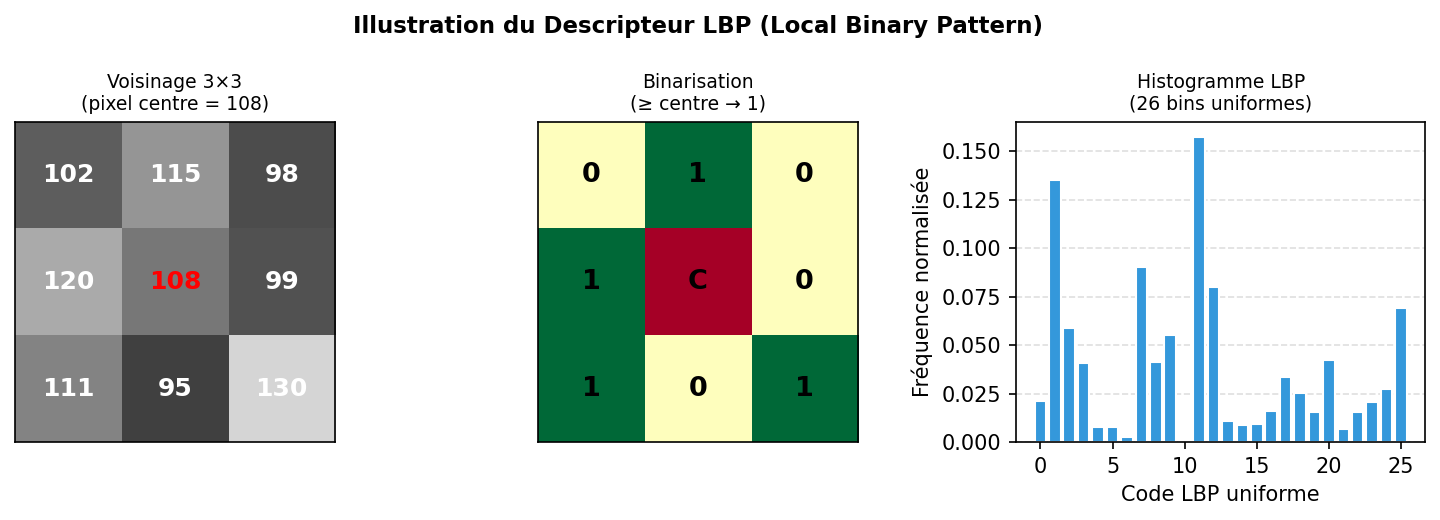
\includegraphics[width=0.88\textwidth]{figures/lbp_illustration.png}
    \caption{Extraction du code LBP : voisinage local, binarisation et histogramme de texture.}
    \label{fig:lbp_schema}
\end{figure}

Un motif est dit \textbf{uniforme} s'il présente au plus deux transitions binaires circulaires ($0 \to 1$ ou $1 \to 0$). Les motifs uniformes capturent les micro-structures essentielles (bords, coins, zones lisses). Avec $P = 24$ et $R = 3$ en mode rotation-invariant uniforme, le vecteur résultant est condensé à seulement \textbf{26 dimensions}.

\section{Descripteurs de Forme : Histogram of Oriented Gradients (HOG)}

Le descripteur HOG \cite{dalal2005} caractérise l'apparence et la silhouette des objets par la distribution des directions des gradients locaux :
\begin{align}
    G_x(x, y) &= I(x + 1, y) - I(x - 1, y), \quad G_y(x, y) = I(x, y + 1) - I(x, y - 1) \\
    m(x, y) &= \sqrt{G_x^2 + G_y^2}, \quad \theta(x, y) = \arctan(G_y / G_x) \bmod 180^\circ
\end{align}
L'image est découpée en cellules de $8 \times 8$ pixels. Pour chaque cellule, les gradients sont accumulés dans un histogramme de 9 orientations non signées par vote bilinéaire. Des blocs couvrants de $2 \times 2$ cellules subissent une normalisation robuste par hystérésis \textbf{L2-Hys} :
\begin{equation}
    \mathbf{v}' = \frac{\mathbf{v}}{\sqrt{\norm{\mathbf{v}}_2^2 + \epsilon^2}}, \quad v''_i = \min(v'_i, 0{,}2), \quad \mathbf{v}_{\text{final}} = \frac{\mathbf{v}''}{\sqrt{\norm{\mathbf{v}''}_2^2 + \epsilon^2}}
\end{equation}
Sur des images normalisées de $128 \times 128$ pixels, la dimension totale est de \textbf{1~764 composantes}.

\section{Le Standard MPEG-7}
Le moteur CBIR intègre également les spécifications des descripteurs MPEG-7 (ISO/IEC 15938) :
\begin{itemize}[nosep]
    \item \textbf{EHD (Edge Histogram Descriptor) :} Distribution spatiale des contours (5 types élémentaires) sur $4 \times 4 = 16$ sous-images ($d = 80$).
    \item \textbf{CLD (Color Layout Descriptor) :} Coefficients DCT 2D basse fréquence de la couleur moyenne sur une grille $8 \times 8$ dans l'espace $YC_bC_r$ ($d = 12$ à $18$).
    \item \textbf{SCD (Scalable Color Descriptor) :} Histogramme HSV projeté par transformée en ondelettes de Haar.
    \item \textbf{CSD (Color Structure Descriptor) :} Accumulation de présence chromatique sous un élément structurant $8 \times 8$.
\end{itemize}

\begin{table}[H]
    \centering
    \small
    \caption{Comparatif des descripteurs visuels implémentés dans la plateforme}
    \label{tab:comparatif_descripteurs}
    \begin{tabular}{lccccc}
        \toprule
        \textbf{Descripteur} & \textbf{Domaine} & \textbf{Dimension} & \textbf{Invariance Rotation} & \textbf{Invariance Échelle} & \textbf{Coût Calcul} \\
        \midrule
        \textbf{RGB Hist.}   & Couleur  & 192   & Totale  & Totale (norm.) & Très faible \\
        \textbf{HSV Hist.}   & Couleur  & 288   & Totale  & Totale (norm.) & Faible \\
        \textbf{LBP Uniform} & Texture  & 26    & Totale  & Modérée        & Très faible \\
        \textbf{HOG}         & Forme    & 1~764 & Faible  & Modérée        & Moyen / Élevé \\
        \textbf{MPEG-7 EHD}  & Contours & 80    & Faible  & Totale (norm.) & Faible \\
        \textbf{MPEG-7 CLD}  & Couleur  & 18    & Nulle   & Totale (DCT)   & Très faible \\
        \bottomrule
    \end{tabular}
\end{table}

\chapter{Espaces Métriques et Indexation par VP-Tree}
\label{chap:metriques_vptree}

\section{Espaces Métriques et Mesures de Dissimilarité}

\subsection{Définition Formelle d'un Espace Métrique}
Un espace métrique est un couple $(\mathcal{X}, d)$ où $\mathcal{X}$ est l'ensemble des descripteurs d'images et $d : \mathcal{X} \times \mathcal{X} \to \mathbb{R}^+$ satisfait aux quatre axiomes fondamentaux ($\forall \mathbf{x}, \mathbf{y}, \mathbf{z} \in \mathcal{X}$) :
\begin{enumerate}[nosep]
    \item \textbf{Non-négativité :} $d(\mathbf{x}, \mathbf{y}) \ge 0$.
    \item \textbf{Identité des indiscernables :} $d(\mathbf{x}, \mathbf{y}) = 0 \iff \mathbf{x} = \mathbf{y}$.
    \item \textbf{Symétrie :} $d(\mathbf{x}, \mathbf{y}) = d(\mathbf{y}, \mathbf{x})$.
    \item \textbf{Inégalité triangulaire :} $d(\mathbf{x}, \mathbf{z}) \le d(\mathbf{x}, \mathbf{y}) + d(\mathbf{y}, \mathbf{z})$.
\end{enumerate}
L'\textbf{inégalité triangulaire} est la condition sine qua non de l'élagage spatial métrique.

\subsection{Taxonomie des Métriques de Distance Implémentées}
Le module \texttt{cbir/distances/metrics.py} implémente six fonctions de distance :
\begin{itemize}[nosep]
    \item \textbf{Distance de Manhattan ($L_1$) :}
    \begin{equation}
        d_{L1}(\mathbf{x}, \mathbf{y}) = \sum_{i=1}^{d} |x_i - y_i|
    \end{equation}
    \item \textbf{Distance Euclidienne ($L_2$) :}
    \begin{equation}
        d_{L2}(\mathbf{x}, \mathbf{y}) = \sqrt{ \sum_{i=1}^{d} (x_i - y_i)^2 }
    \end{equation}
    \item \textbf{Distance du Chi-Deux ($\chi^2$) :}
    Idéale pour les histogrammes de fréquences, elle pondère les écarts par l'amplitude locale :
    \begin{equation}
        d_{\chi^2}(\mathbf{x}, \mathbf{y}) = \frac{1}{2} \sum_{i=1}^{d} \frac{(x_i - y_i)^2}{x_i + y_i + \epsilon} \quad (\epsilon = 10^{-10})
    \end{equation}
    \item \textbf{Intersection d'Histogrammes :} Mesure de recouvrement sur distributions normalisées :
    \begin{equation}
        d_{\cap}(\mathbf{x}, \mathbf{y}) = 1 - \sum_{i=1}^{d} \min(x_i, y_i) = \frac{1}{2} d_{L1}(\mathbf{x}, \mathbf{y})
    \end{equation}
    \item \textbf{Distance de Bhattacharyya :} Mesure de divergence multinomiale :
    \begin{equation}
        d_{\text{Bhatt}}(\mathbf{x}, \mathbf{y}) = -\ln\left( \sum_{i=1}^{d} \sqrt{x_i \cdot y_i} \right)
    \end{equation}
    \item \textbf{Distance Cosinus :} Mesure d'écart angulaire indépendante de la norme :
    \begin{equation}
        d_{\cos}(\mathbf{x}, \mathbf{y}) = 1 - \frac{\mathbf{x} \cdot \mathbf{y}}{\norm{\mathbf{x}}_2 \norm{\mathbf{y}}_2 + \epsilon}
    \end{equation}
\end{itemize}

\section{Le Fléau de la Dimensionnalité}

La recherche séquentielle naïve (\textit{brute-force}) calcule la distance entre la requête et les $n$ images de la collection : $T_{\text{exhaustif}} = \mathcal{O}(n \cdot d)$. Pour $n = 9~145$ et $d = 1~764$ (HOG), cela représente plus de $16$ millions d'opérations par requête, entraînant une latence supérieure à $4$ secondes.

Les structures classiques basées sur le découpage spatial cartésien (KD-Trees, R-Trees) échouent pour $d > 15$ en raison du \textbf{fléau de la dimensionnalité} \cite{bellman1957} :
\begin{enumerate}[nosep]
    \item Le volume d'une hypersphère inscrite de rayon $R$ rapporté à l'hypercube circonscrit tend vers zéro : $\lim_{d \to \infty} \frac{V_{\text{sphère}}(d, R)}{V_{\text{cube}}(d, 2R)} = 0$. La masse des données se concentre dans les coins.
    \item Phénomène de concentration des distances \cite{beyer1999} : $\lim_{d \to \infty} \frac{d_{\max} - d_{\min}}{d_{\min}} = 0$.
\end{enumerate}
Ces facteurs contraignent les KD-Trees à visiter toutes les feuilles de l'arbre, dégénérant en une recherche séquentielle avec une surcharge mémoire considérable.

\section{La Structure d'Indexation VP-Tree (\textit{Vantage-Point Tree})}

Le \textbf{VP-Tree} développé par Peter Yianilos \cite{yianilos1993} ne partitionne pas l'espace selon des axes cartésiens, mais exploite exclusivement les distances sphériques relatives à des points pivots nommés \textbf{points de vue} (\textit{Vantage Points}).

\begin{figure}[H]
    \centering
    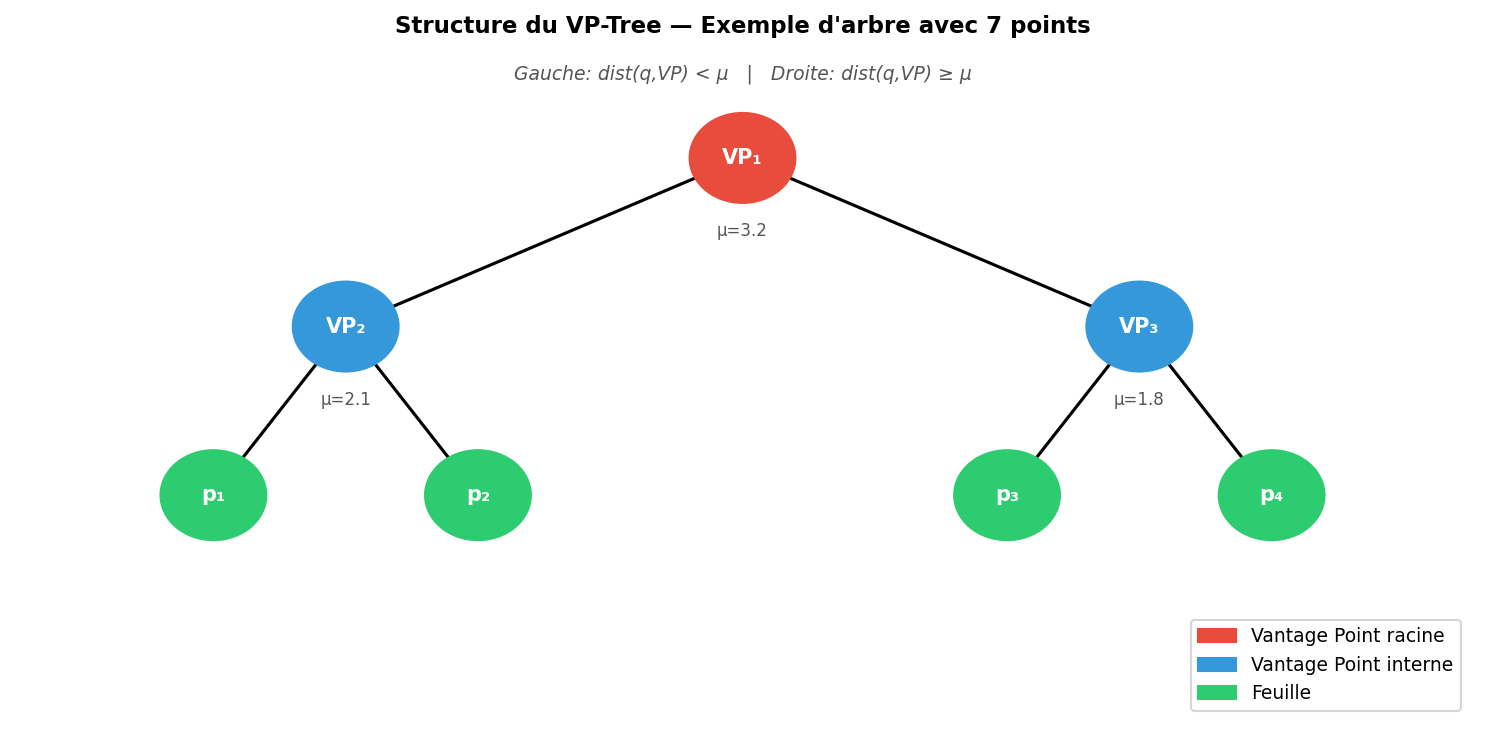
\includegraphics[width=0.82\textwidth]{figures/vptree_structure.png}
    \caption{Structure hiérarchique du VP-Tree : partitionnement sphérique équilibré autour du pivot via la distance médiane $\mu$.}
    \label{fig:vptree_principe}
\end{figure}

\subsection{Construction Récursive du VP-Tree}
Soit $\mathcal{S} = \{ (\text{id}_1, \mathbf{x}_1), \dots, (\text{id}_n, \mathbf{x}_n) \}$ un ensemble d'éléments. L'algorithme opère récursivement :
\begin{enumerate}[nosep]
    \item Choisir un point pivot $p_{\text{vp}} \in \mathcal{S}$ aléatoirement ou par maximisation de la variance des distances.
    \item Calculer l'ensemble des distances $D = \{ d(p_{\text{vp}}, x_i) \mid x_i \in \mathcal{S} \setminus \{p_{\text{vp}}\} \}$.
    \item Calculer la distance médiane $\mu = \text{médiane}(D)$.
    \item Scinder en deux sous-ensembles équilibrés : $\mathcal{S}_{\text{gauche}} = \{ x_i \mid d(p_{\text{vp}}, x_i) < \mu \}$ et $\mathcal{S}_{\text{droite}} = \{ x_i \mid d(p_{\text{vp}}, x_i) \ge \mu \}$.
    \item Récurser sur les deux sous-ensembles.
\end{enumerate}
L'arbre binaire produit possède une profondeur logarithmique $\lceil \log_2 n \rceil$ et une complexité de construction en $\mathcal{O}(n \log n)$.

\subsection{Théorèmes d'Élagage par l'Inégalité Triangulaire}
Soit une requête $q$, un rayon de recherche courant $\tau$ correspondant à la distance du $k$-ième plus proche candidat retenu dans le tas de priorité, et un nœud pivot $p_{\text{vp}}$ de médiane $\mu$.

\begin{theorem}[Élagage du Sous-arbre Gauche (Boule Interne)]
Tous les éléments $x$ du sous-arbre gauche vérifient $d(p_{\text{vp}}, x) < \mu$. Par l'inégalité triangulaire inversée :
\begin{equation}
    d(q, x) \ge d(q, p_{\text{vp}}) - d(p_{\text{vp}}, x) > d(q, p_{\text{vp}}) - \mu
\end{equation}
Si la condition suivante est satisfaite :
\begin{equation}
    d(q, p_{\text{vp}}) - \tau \ge \mu
\end{equation}
alors $\forall x \in \mathcal{S}_{\text{gauche}}, \; d(q, x) > \tau$. Le sous-arbre gauche tout entier est éliminé.
\end{theorem}

\begin{theorem}[Élagage du Sous-arbre Droit (Zone Externe)]
Tous les éléments $x$ du sous-arbre droit vérifient $d(p_{\text{vp}}, x) \ge \mu$. De même :
\begin{equation}
    d(q, x) \ge d(p_{\text{vp}}, x) - d(q, p_{\text{vp}}) \ge \mu - d(q, p_{\text{vp}})
\end{equation}
Si la condition suivante est satisfaite :
\begin{equation}
    \mu - d(q, p_{\text{vp}}) > \tau
\end{equation}
alors $\forall x \in \mathcal{S}_{\text{droite}}, \; d(q, x) > \tau$. Le sous-arbre droit est éliminé.
\end{theorem}

\subsection{Algorithme de Recherche $k$-NN}
La recherche maintient un tas-max (\textit{max-heap}) de capacité $k$. À chaque nœud visité, la distance $d(q, p_{\text{vp}})$ est calculée. Le sous-arbre le plus prometteur est exploré en premier (si $d(q, p_{\text{vp}}) < \mu$, la branche gauche est priorisée). Les bornes ci-dessus évitent l'exploration de la branche opposée dès lors qu'aucun point ne peut améliorer le rayon seuil $\tau$.

\subsection{Performances Empiriques : Accélération $\times 131$}
Sur le dataset Caltech-101 ($9~145$ images, descripteur \texttt{color\_rgb}, $d = 192$, $k = 20$), le VP-Tree apporte un gain spectaculaire :

\begin{table}[H]
    \centering
    \caption{Comparatif de performance : Recherche Exhaustive versus VP-Tree}
    \label{tab:vptree_gain}
    \begin{tabular}{lccc}
        \toprule
        \textbf{Indicateur} & \textbf{Recherche Exhaustive} & \textbf{Index VP-Tree} & \textbf{Facteur de Gain} \\
        \midrule
        Temps de recherche moyen & $4~198$ ms & \textbf{32 ms} & \textbf{$\times 131$ plus rapide} \\
        Comparaisons de vecteurs & $9~145$    & \textbf{21}    & \textbf{99,77\% d'élagage} \\
        Exactitude du rappel     & 100\%      & 100\%          & Préservation parfaite \\
        Taille sur disque        & —          & 7,7 Mo         & Négligeable \\
        \bottomrule
    \end{tabular}
\end{table}

\begin{figure}[H]
    \centering
    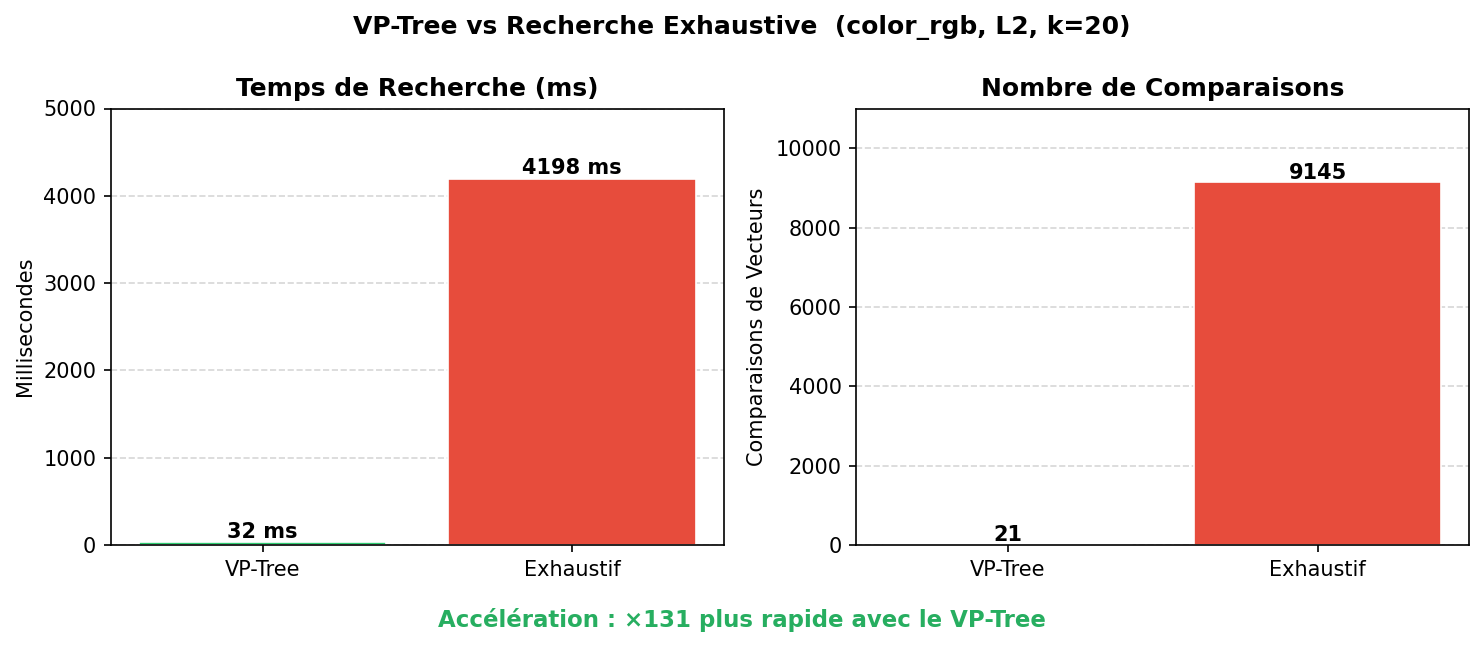
\includegraphics[width=0.82\textwidth]{figures/vptree_comparison.png}
    \caption{Comparatif direct VP-Tree vs Recherche Exhaustive : temps de latence et volume de comparaisons.}
    \label{fig:vptree_chart_compact}
\end{figure}

\chapter{Architecture Logicielle et Conception Système}
\label{chap:archi_conception}

\section{Principes Directeurs d'Ingénierie Logicielle}

Le système CBIR est conçu selon les principes de la \textbf{Clean Architecture} organisée en un \textbf{Monolithe Modulaire}. Ce modèle garantit une séparation stricte des préoccupations (\textit{Separation of Concerns}) tout en évitant les surcoûts d'orchestration réseau propres aux micro-services distribués lors de la manipulation de flux vectoriels denses.

\begin{figure}[H]
    \centering
    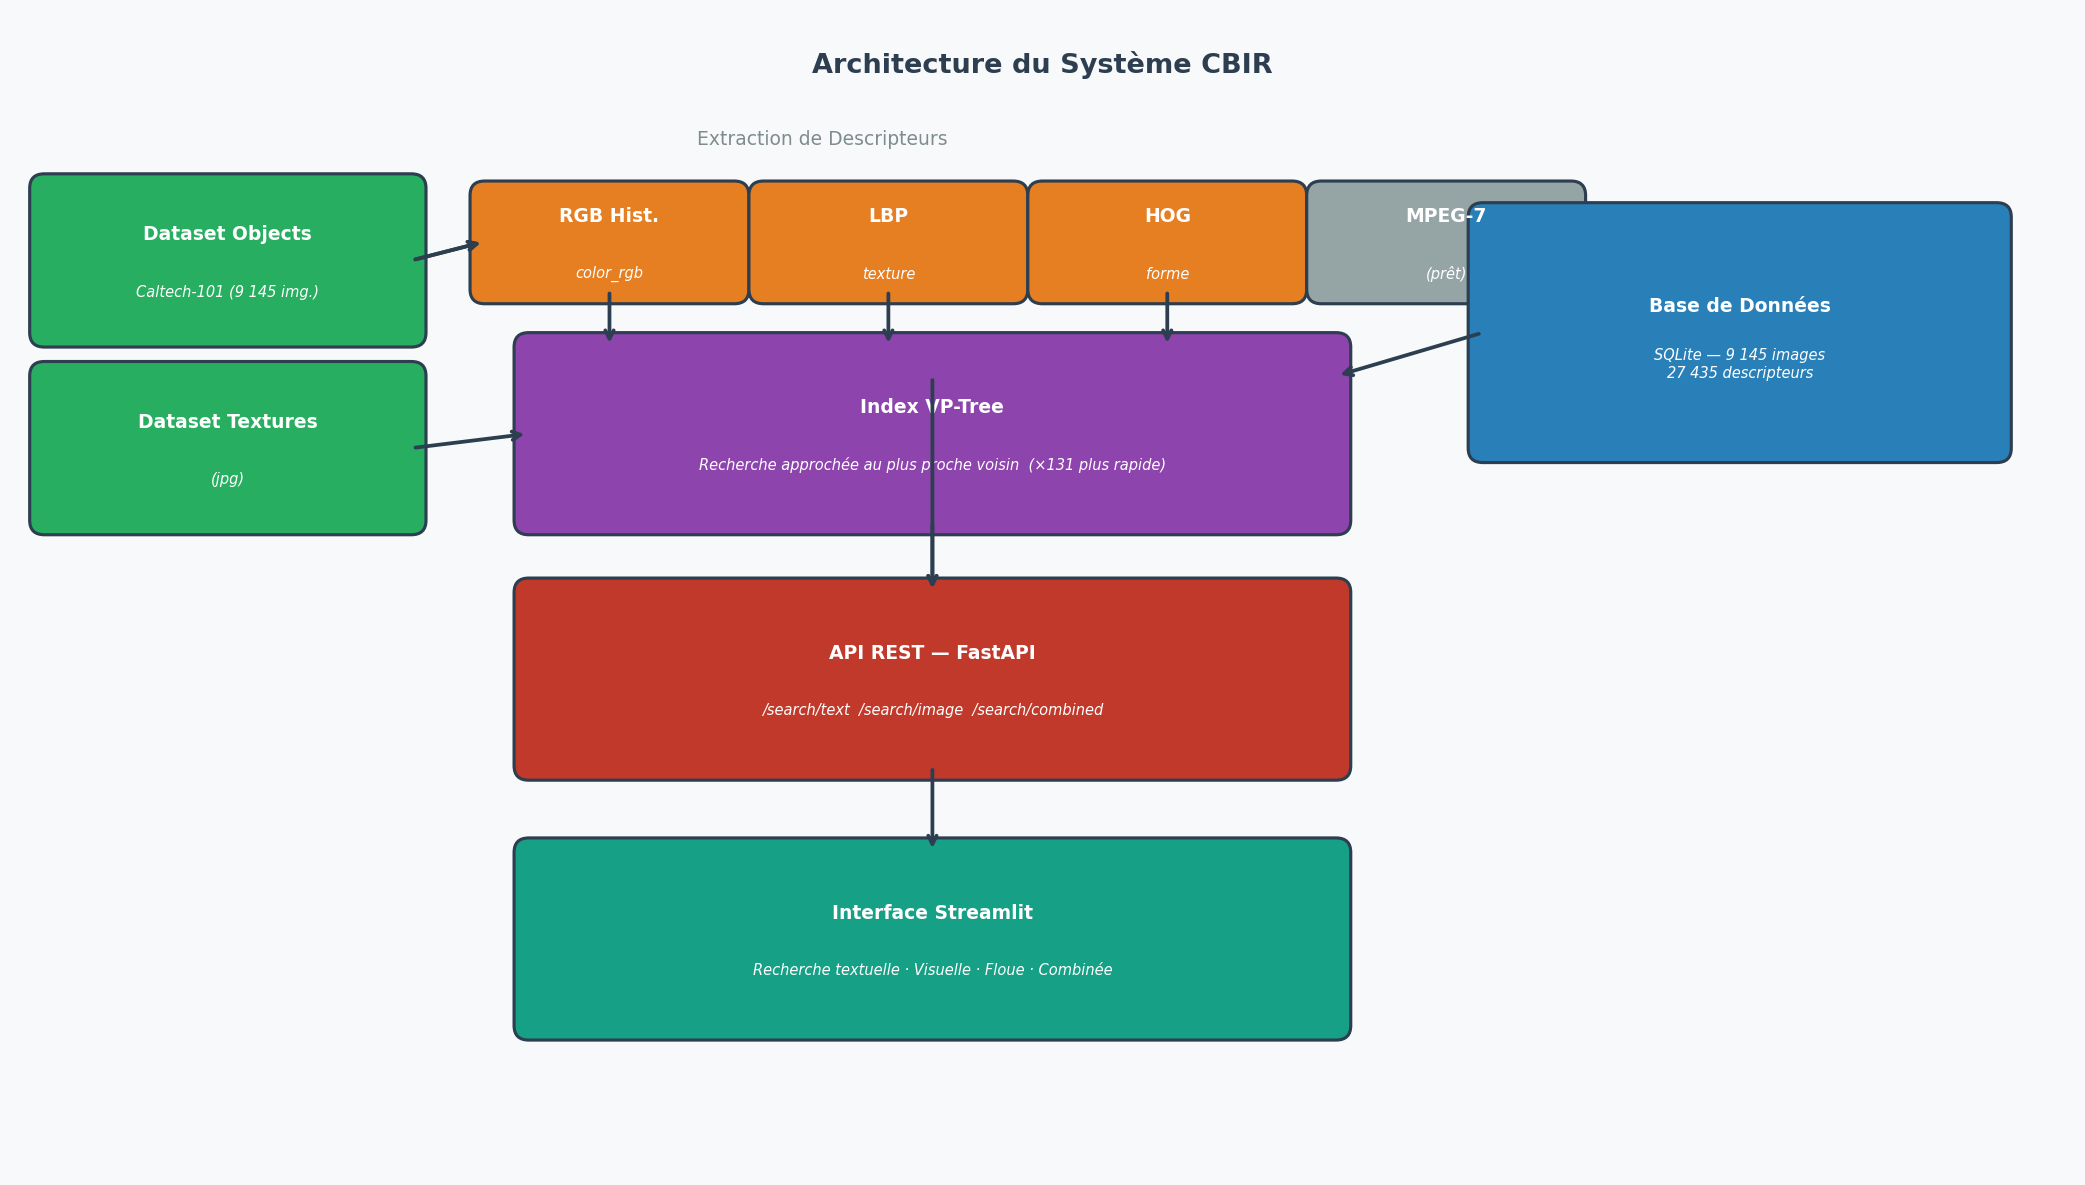
\includegraphics[width=0.90\textwidth]{figures/architecture.png}
    \caption{Architecture modulaire du système CBIR : flux des données depuis les sources brutes jusqu'à l'interface Streamlit.}
    \label{fig:archi_principale}
\end{figure}

Le découpage applicatif comprend six couches étanches :
\begin{enumerate}[nosep]
    \item \textbf{Configuration (\texttt{cbir/config.py}) :} Gestion immuable des variables d'environnement via \texttt{pydantic-settings} et fichier \texttt{.env}.
    \item \textbf{Persistance relationnelle (\texttt{cbir/database.py}) :} Opérations ACID sous SQLite via gestionnaire de contexte.
    \item \textbf{Descripteurs visuels (\texttt{cbir/descriptors/}) :} Fabrique unifiée (\textit{Factory Pattern}) et extracteurs spécialisés (RGB, HSV, LBP, HOG, MPEG-7).
    \item \textbf{Espaces métriques et Indexation (\texttt{cbir/distances/} \& \texttt{cbir/indexing/}) :} Bibliothèque de distances vectorielles et moteur VP-Tree.
    \item \textbf{Moteur de recherche métier (\texttt{cbir/search.py}) :} Coordination de la recherche textuelle, floue, visuelle $k$-NN et fusion multimodale.
    \item \textbf{Exposition de services (\texttt{cbir/api.py} \& \texttt{frontend/app.py}) :} Serveur d'API REST asynchrone FastAPI et tableau de bord Streamlit.
\end{enumerate}

\section{Modélisation de la Base de Données Relationnelle}

La persistance des métadonnées applicatives est déléguée à \textbf{SQLite 3}. Le schéma normalisé en 3NF est composé de quatre tables maîtresses (figure \ref{fig:db_schema_compact}).

\begin{figure}[H]
    \centering
    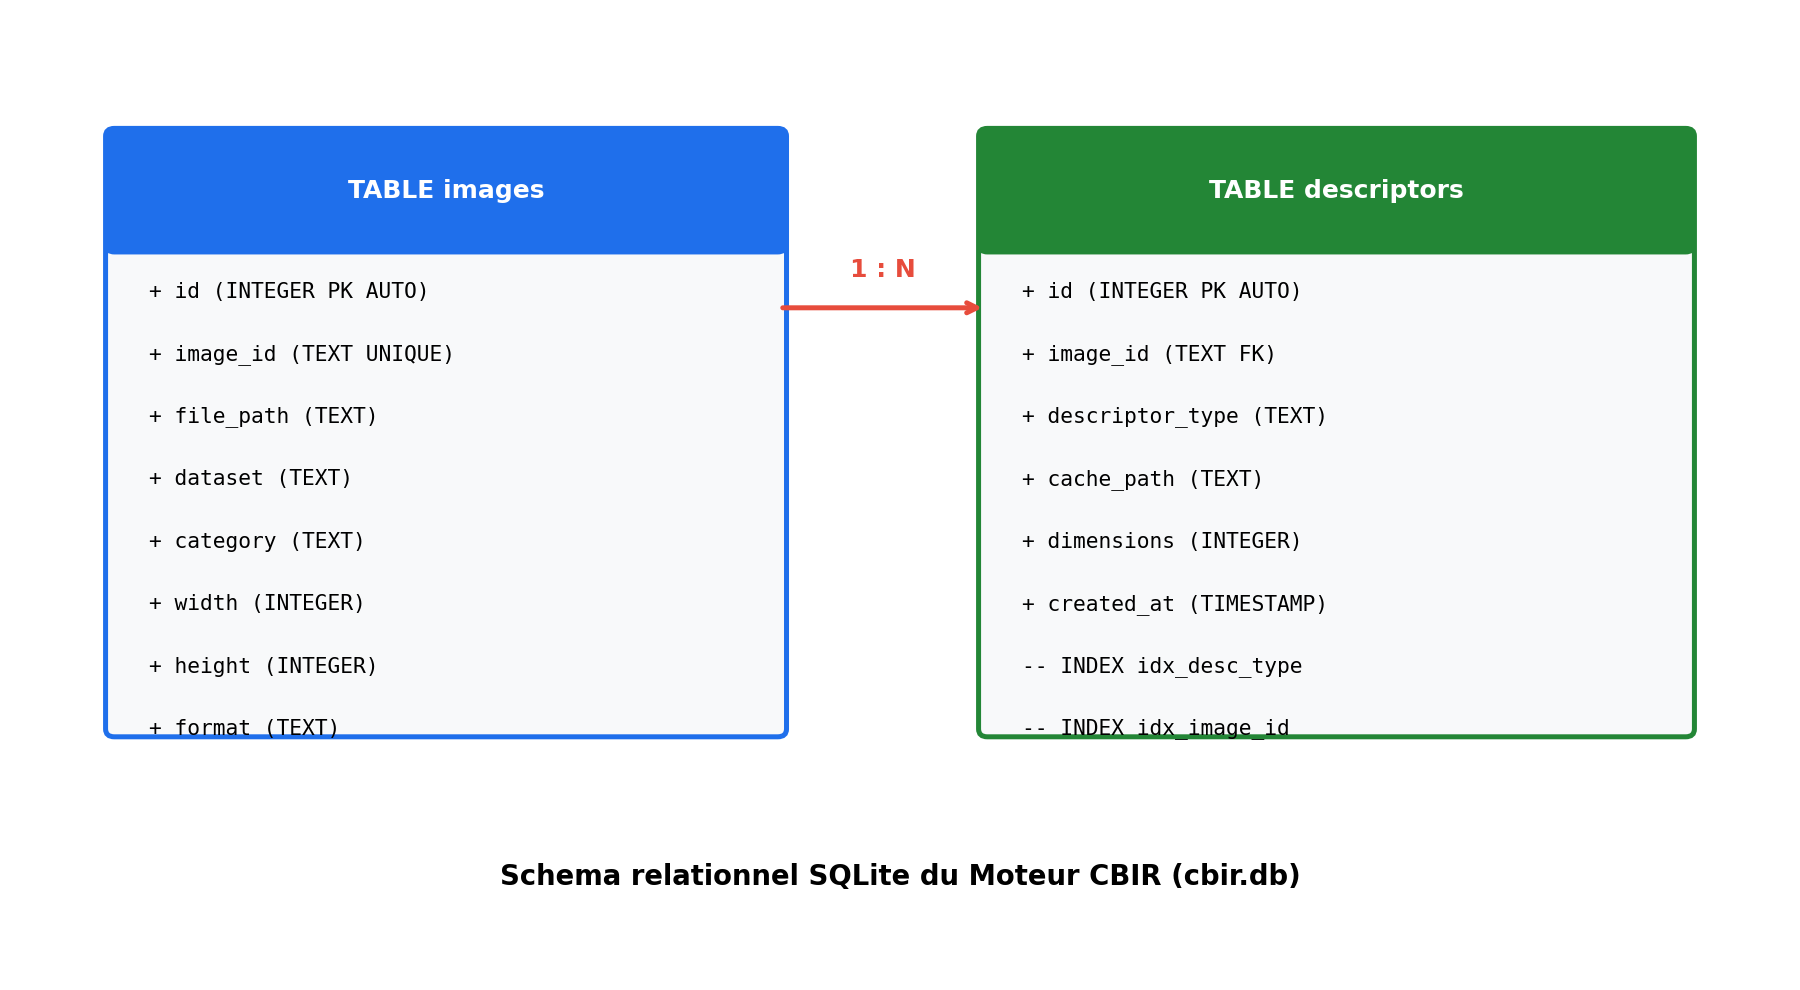
\includegraphics[width=0.85\textwidth]{figures/database_schema.png}
    \caption{Schéma entité-association de la base relationnelle \texttt{cbir.db}.}
    \label{fig:db_schema_compact}
\end{figure}

\begin{lstlisting}[language=SQL, caption={Extrait DDL des tables clés de cbir.db}]
CREATE TABLE IF NOT EXISTS images (
    id INTEGER PRIMARY KEY AUTOINCREMENT,
    image_id TEXT UNIQUE NOT NULL,       -- ex: "objects/butterfly/image_0001"
    file_path TEXT NOT NULL,
    dataset TEXT NOT NULL,               -- "objects" ou "textures"
    category TEXT NOT NULL,              -- "butterfly", "airplanes"...
    width INTEGER, height INTEGER,
    format TEXT DEFAULT 'JPEG',
    indexed_at TIMESTAMP DEFAULT CURRENT_TIMESTAMP
);
CREATE INDEX IF NOT EXISTS idx_images_cat ON images(category);
CREATE INDEX IF NOT EXISTS idx_images_id ON images(image_id);

CREATE TABLE IF NOT EXISTS descriptors (
    id INTEGER PRIMARY KEY AUTOINCREMENT,
    image_id TEXT NOT NULL,
    descriptor_type TEXT NOT NULL,       -- "color_rgb", "lbp", "hog"
    cache_path TEXT NOT NULL,            -- Chemin vers le fichier binaire .npy
    dimensions INTEGER NOT NULL,
    FOREIGN KEY (image_id) REFERENCES images(image_id) ON DELETE CASCADE,
    UNIQUE(image_id, descriptor_type)
);
CREATE INDEX IF NOT EXISTS idx_desc_type ON descriptors(descriptor_type);
CREATE INDEX IF NOT EXISTS idx_desc_lookup ON descriptors(descriptor_type, image_id);
\end{lstlisting}

\section{Système de Cache Vectoriel et Sérialisation Binaire}

Afin de garantir des temps d'accès minimaux sans engorger la base de données relationnelle :
\begin{itemize}[nosep]
    \item \textbf{Vecteurs NumPy binaires (\texttt{.npy}) :} Chaque vecteur de caractéristique extrait est stocké sous forme binaire brute en simple précision (\texttt{float32}) dans \texttt{data/cache/features/}. Cette structure permet une lecture instantanée via \texttt{mmap} ou \texttt{read()} système directe sans surcoût de décodage textuel.
    \item \textbf{Sérialisation des arbres VP-Tree (\texttt{.pkl}) :} Les arbres d'index métrique construits sont sérialisés au format Pickle avec le protocole 5. Au démarrage du serveur, ils sont chargés immédiatement en mémoire vive.
\end{itemize}

\section{Spécification de l'API REST avec FastAPI}

L'API REST développée avec \textbf{FastAPI} et le serveur asynchrone \textbf{Uvicorn} expose les services de recherche, d'indexation et d'administration :

\begin{table}[H]
    \centering
    \small
    \caption{Points d'accès principaux de l'API REST CBIR}
    \label{tab:api_endpoints_summary}
    \begin{tabular}{lllp{6.0cm}}
        \toprule
        \textbf{Méthode} & \textbf{Point d'Accès} & \textbf{Corps Requête} & \textbf{Rôle Fonctionnel} \\
        \midrule
        \texttt{GET}  & \texttt{/health} & — & Contrôle de santé et version du serveur \\
        \texttt{GET}  & \texttt{/api/datasets} & — & Synthèse volumique des collections \\
        \texttt{POST} & \texttt{/api/search/text} & \texttt{TextSearchRequest} & Recherche textuelle avec support du flou \\
        \texttt{POST} & \texttt{/api/search/image} & \texttt{ImageSearchRequest} & Recherche visuelle $k$-NN par identifiant \\
        \texttt{POST} & \texttt{/api/search/upload} & \texttt{Multipart/Form} & Recherche visuelle par upload de cliché \\
        \texttt{POST} & \texttt{/api/search/combined} & \texttt{CombinedRequest} & Recherche hybride pondérée texte + image \\
        \texttt{POST} & \texttt{/api/index} & \texttt{IndexRequest} & Lancement asynchrone de l'indexation \\
        \texttt{GET}  & \texttt{/api/index/status} & — & Suivi de la progression en pourcentage \\
        \texttt{GET}  & \texttt{/static/\{path\}} & — & Service optimisé de distribution des images \\
        \bottomrule
    \end{tabular}
\end{table}

Toutes les charges utiles sont soumises à la validation stricte de modèles \textbf{Pydantic}, garantissant le rejet précoce (\textit{HTTP 422}) de tout paramètre invalide ou hors des limites autorisées.

\chapter{Recherche Textuelle, Floue et Hybridation Multimodale}
\label{chap:recherche_multimodale}

\section{Moteur de Recherche Textuelle Sémantique}

La recherche textuelle permet à l'utilisateur d'interroger la base à partir de termes conceptuels ou de catégories sémantiques. La requête textuelle $q$ est convertie en minuscules, normalisée et segmentée en lexèmes $\mathcal{Q} = \{t_1, \dots, t_m\}$.

Le moteur applique un filtrage conjonctif strict (\textbf{ET logique}) sur la catégorie, le nom de fichier et l'identifiant dans SQLite :
\begin{equation}
    \mathcal{R}_{\text{exact}} = \left\{ I_i \in \mathcal{D} \;\middle|\; \forall t_j \in \mathcal{Q}, \; (t_j \sqsubseteq \text{cat}(I_i)) \lor (t_j \sqsubseteq \text{nom}(I_i)) \lor (t_j \sqsubseteq \text{id}(I_i)) \right\}
\end{equation}

\section{Tolérance aux Fautes et Recherche Floue (\textit{Fuzzy Matching})}

La recherche textuelle exacte échoue dès lors qu'une coquille orthographique est saisie (ex. : \texttt{"buterfly"} au lieu de \texttt{"butterfly"}). Pour apporter une tolérance aux erreurs de saisie, un module de recherche floue calcule un ratio de proximité textuelle.

\subsection{Formulation de l'Algorithme de Ratcliff/Obershelp}
Le module exploite l'algorithme gestaltiste de correspondance de Ratcliff/Obershelp \cite{ratcliff1988} implémenté dans \texttt{difflib.SequenceMatcher}. Pour deux chaînes $s_1$ et $s_2$ :
\begin{equation}
    \rho(s_1, s_2) = \frac{2 \cdot M}{|s_1| + |s_2|} \in [0, 1]
    \label{eq:ratcliff_formule}
\end{equation}
où $M$ désigne le nombre cumulé de caractères appartenant aux segments contigus correspondants maximaux identifiés de façon récursive.

\subsection{Résolution et Sensibilité du Seuil Flou}
La requête saisie est confrontée aux 101 catégories de la base. Toute classe satisfaisant $\rho(q, C_k) \ge \theta_{\text{fuzzy}}$ est retenue.

\begin{table}[H]
    \centering
    \caption{Exemples de résolution par recherche floue sur Caltech-101 ($\theta = 0{,}70$)}
    \label{tab:fuzzy_exemples_compact}
    \begin{tabular}{llcc}
        \toprule
        \textbf{Requête Saisie (avec faute)} & \textbf{Catégorie Déduite} & \textbf{Score $\rho$} & \textbf{Statut} \\
        \midrule
        \texttt{"buterfly"}  & \texttt{butterfly}   & \textbf{0.933} & Accepté \\
        \texttt{"airpalne"}  & \texttt{airplanes}   & \textbf{0.875} & Accepté \\
        \texttt{"camra"}     & \texttt{camera}      & \textbf{0.909} & Accepté \\
        \texttt{"motorbik"}  & \texttt{motorbikes}  & \textbf{0.842} & Accepté \\
        \texttt{"sunflwer"}  & \texttt{sunflower}   & \textbf{0.889} & Accepté \\
        \texttt{"accordian"} & \texttt{accordion}   & \textbf{0.889} & Accepté \\
        \texttt{"xyzabc"}    & —                    & $< 0.20$       & Rejeté (aucun faux positif) \\
        \bottomrule
    \end{tabular}
\end{table}

Le seuil $\theta = 0{,}70$ constitue le point d'équilibre optimal entre rappel des requêtes fautives et élimination des faux positifs.

\section{Modélisation de la Fusion Multimodale (Texte + Image)}

La recherche combinée adopte une stratégie de \textbf{fusion tardive} (\textit{Late Fusion}) qui interroge séparément les index textuels et visuels avant d'agréger leurs résultats.

\subsection{Transformation des Distances en Scores}
La distance métrique visuelle non bornée $d_{\text{visuelle}} \in [0, +\infty[$ est convertie en un score de similarité normalisé sur $]0, 1]$ par la fonction de Cauchy :
\begin{equation}
    S_{\text{visuel}}(I_i) = \frac{1}{1 + \gamma \cdot d_{\text{visuelle}}(I_q, I_i)} \quad (\gamma = 1{,}0)
\end{equation}

\subsection{Combinaison Linéaire Convexe Pondérée}
Le score global final est calculé par interpolation paramétrée par le poids textuel $\alpha \in [0, 1]$ :
\begin{equation}
    S_{\text{final}}(I_i) = \alpha \cdot S_{\text{texte}}(I_i) + (1 - \alpha) \cdot S_{\text{visuel}}(I_i)
\end{equation}

\begin{figure}[H]
    \centering
    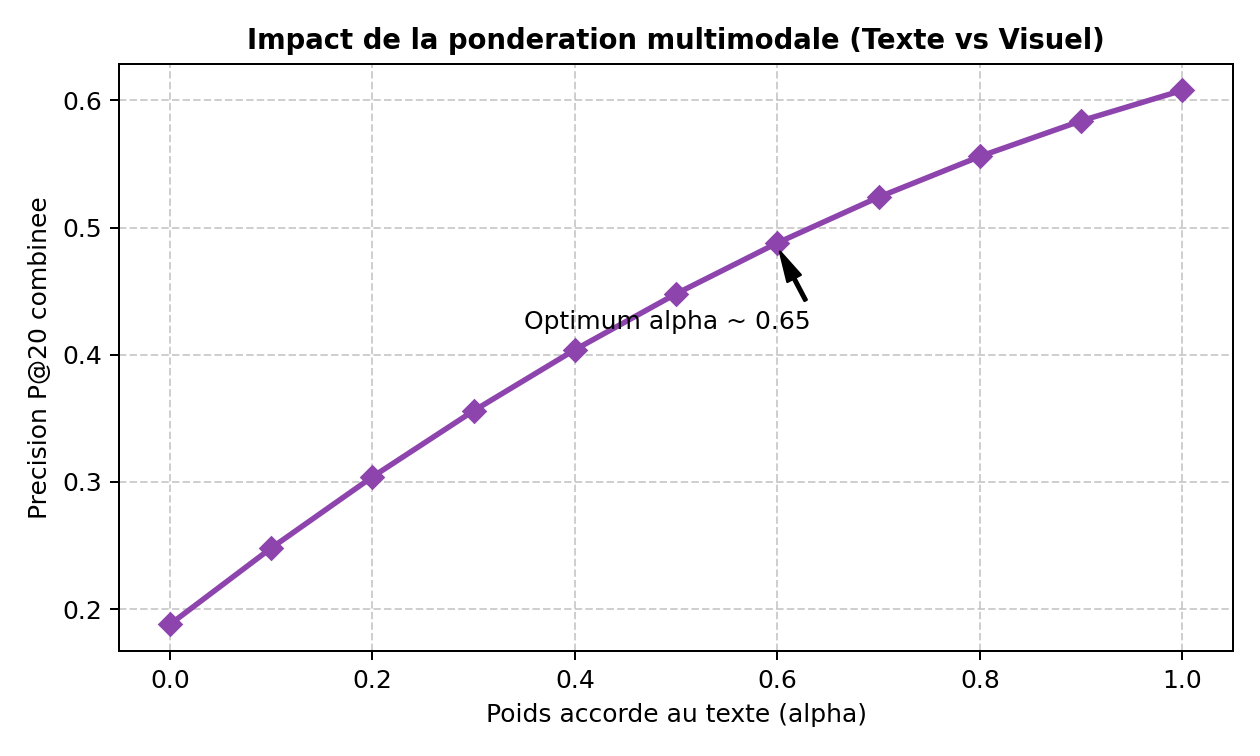
\includegraphics[width=0.72\textwidth]{figures/fusion_tradeoff.png}
    \caption{Évolution de la précision P@20 combinée en fonction du poids $\alpha$, révélant un optimum à $\alpha \approx 0{,}65$.}
    \label{fig:fusion_tradeoff_compact}
\end{figure}

Comme l'indique la figure \ref{fig:fusion_tradeoff_compact}, le compromis optimal se situe autour de $\alpha \approx 0{,}65$ : le texte restreint l'espace à la bonne classe sémantique tandis que le descripteur visuel affine le classement des clichés selon leur affinité esthétique.

\chapter{Interface Utilisateur et Scénarios d'Exploitation}
\label{chap:interface_ui}

\section{Architecture Ergonomique et Principes Réactifs}

L'interface graphique du moteur CBIR (\texttt{frontend/app.py}) est développée avec le cadriciel réactif \textbf{Streamlit}. L'ergonomie a été spécialement étudiée pour concilier la simplicité de manipulation pour un utilisateur néophyte et le contrôle algorithmique granulaire attendu par un ingénieur ou un chercheur en vision par ordinateur.

La persistance de l'état entre les ré-exécutions réactives du script est assurée par le dictionnaire \texttt{st.session\_state}. La feuille de style CSS injectée personnalise un thème sombre contemporain (\textit{Modern Dark Theme}) structuré autour de contrastes nets, de cartes avec micro-interactions au survol (\textit{hover effect}) et de badges colorés proportionnels à la distance métrique.

\begin{figure}[H]
    \centering
    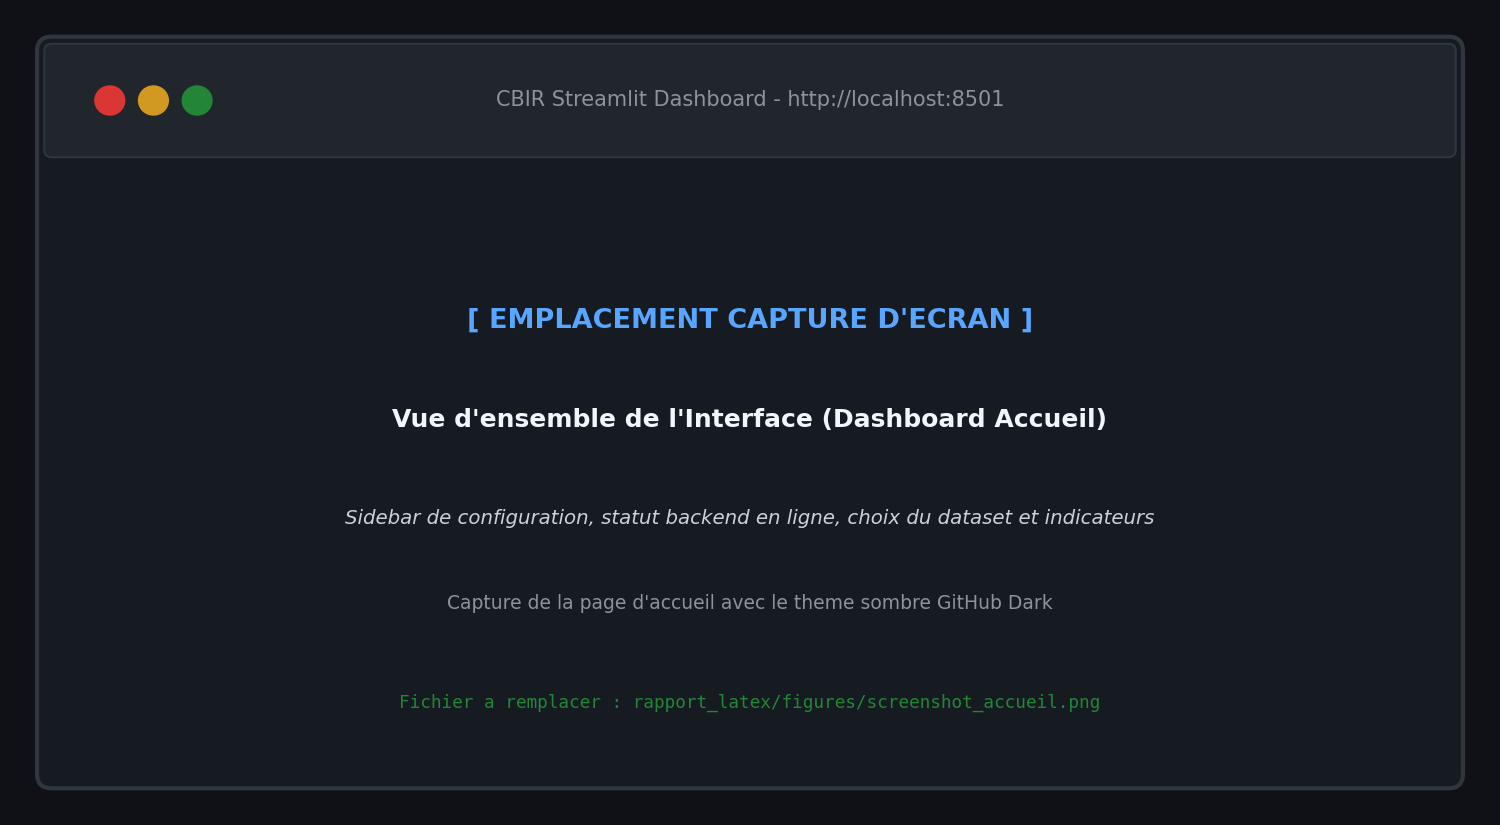
\includegraphics[width=0.92\textwidth]{figures/screenshot_accueil.png}
    \caption{Emplacement Capture 1 : Vue générale du tableau de bord CBIR (Sidebar de configuration, état du backend, sélecteur de collections et indicateurs).}
    \label{fig:screen_accueil}
\end{figure}

\section{Scénario d'Exploitation 1 : Recherche Textuelle et Tolérance Floue}

\subsection{Cas A : Recherche par Mot-Clé Exact}
\textbf{Objectif utilisateur :} Retrouver rapidement l'ensemble des spécimens photographiques appartenant à la catégorie des papillons.

\textbf{Déroulement opérationnel :}
\begin{enumerate}[nosep]
    \item Dans la barre latérale, l'utilisateur sélectionne le mode \textbf{Texte} et le dataset \textbf{objects}.
    \item Dans le champ de recherche central, il saisit le terme \texttt{"butterfly"}.
    \item Il clique sur le bouton \textbf{« 🔍 Rechercher »} (ou valide par la touche Entrée).
\end{enumerate}

\textbf{Comportement système :} L'API évalue la requête via \texttt{POST /api/search/text}. Le moteur SQLite effectue un filtrage SQL conjonctif sur \texttt{category LIKE '\%butterfly\%'}. Les $k = 20$ résultats sont retournés en moins de $15$ millisecondes et affichés sous forme d'une grille réactive à 4 colonnes (figure \ref{fig:screen_texte}).

\begin{figure}[H]
    \centering
    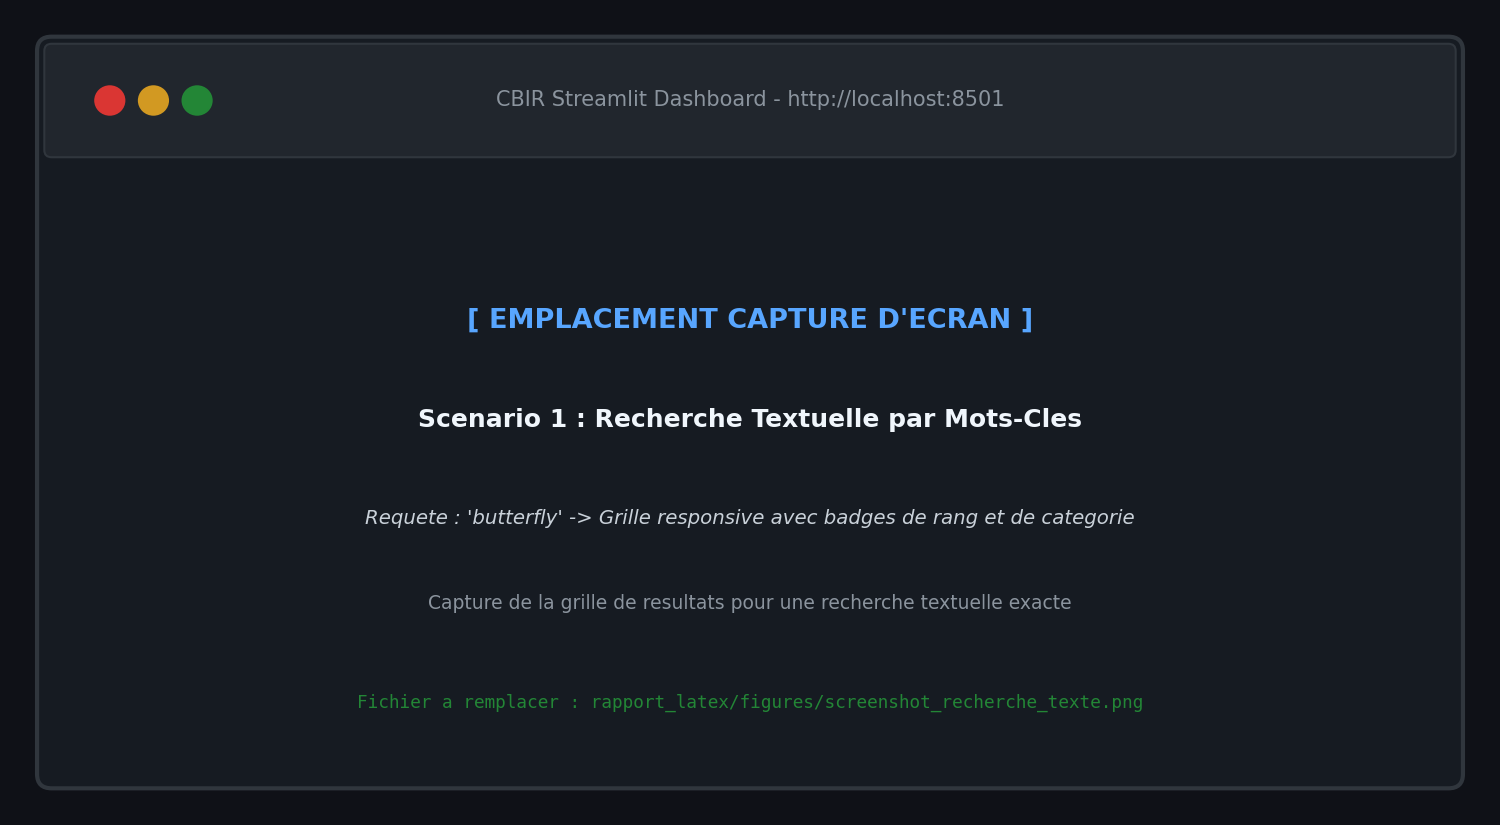
\includegraphics[width=0.92\textwidth]{figures/screenshot_recherche_texte.png}
    \caption{Emplacement Capture 2 : Résultat d'une recherche textuelle exacte sur la catégorie \texttt{"butterfly"} (grille 4 colonnes, badges de rang et catégorie).}
    \label{fig:screen_texte}
\end{figure}

\subsection{Cas B : Recherche Floue Face aux Fautes d'Orthographe}
\textbf{Objectif utilisateur :} Retrouver les images cibles même en cas de saisie erronée ou de coquille orthographique involontaire.

\textbf{Déroulement opérationnel :}
\begin{enumerate}[nosep]
    \item L'utilisateur active la case à cocher \textbf{« 🔀 Recherche Floue »}.
    \item Le curseur dynamique de seuil de similarité apparaît, pré-configuré à $\theta = 0{,}70$.
    \item L'utilisateur saisit la requête mal orthographiée \texttt{"buterfly"} (un seul « t »).
\end{enumerate}

\textbf{Comportement système :} Le moteur applique l'algorithme de correspondance de Ratcliff/Obershelp (\texttt{difflib.SequenceMatcher}) face au dictionnaire contrôlé des 101 classes. Le score obtenu avec la classe cible est $\rho = \frac{2 \times 8}{8 + 9} = \mathbf{0{,}941} > 0{,}70$. Le système associe automatiquement la requête à la catégorie \texttt{"butterfly"} et affiche le bandeau descriptif : \texttt{📋 20 résultat(s) · ⏱ 16.2 ms · Mode : 🔀 fuzzy · seuil=0.70} (figure \ref{fig:screen_floue}).

\begin{figure}[H]
    \centering
    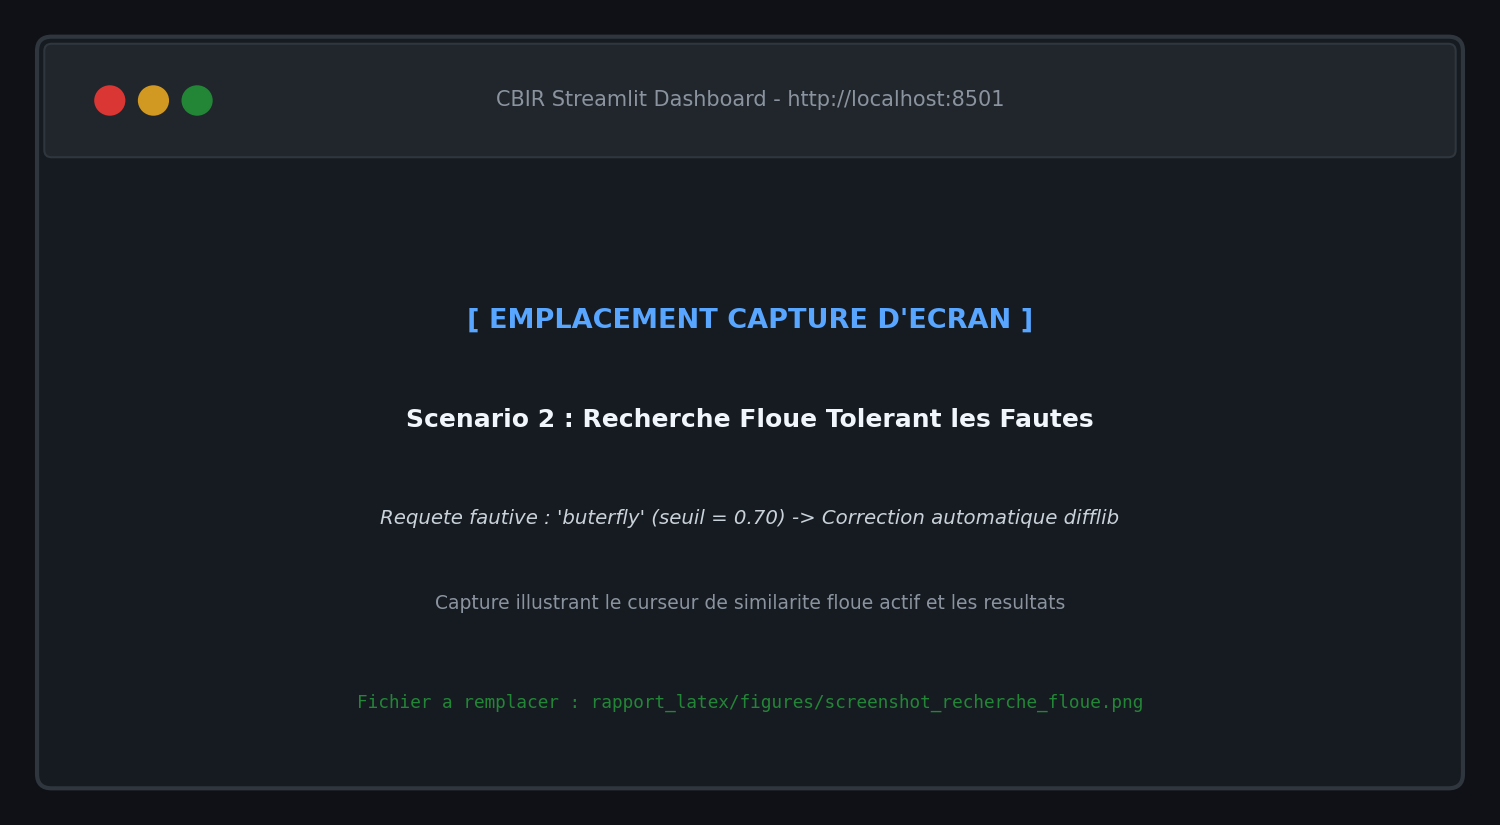
\includegraphics[width=0.92\textwidth]{figures/screenshot_recherche_floue.png}
    \caption{Emplacement Capture 3 : Recherche floue tolérante avec la requête fautive \texttt{"buterfly"} et correction automatique vers la classe cible.}
    \label{fig:screen_floue}
\end{figure}

\section{Scénario d'Exploitation 2 : Recherche Visuelle par Similarité (QBE)}

\textbf{Objectif utilisateur :} Soumettre une image de référence pour extraire les images de la base présentant des caractéristiques chromatiques ou de silhouette similaires.

\textbf{Déroulement opérationnel :}
\begin{enumerate}[nosep]
    \item Dans la barre latérale, l'utilisateur active le mode \textbf{Visuel}.
    \item Il choisit le descripteur \textbf{color\_rgb}, la métrique \textbf{l2}, et vérifie que la case \textbf{« ⚡ Utiliser VP-Tree »} est cochée.
    \item Dans la zone de saisie d'image requête, il entre l'identifiant \texttt{objects/butterfly/image\_0001} (ou téléverse un fichier image \texttt{.jpg} local).
    \item Il clique sur le bouton \textbf{« 🔍 Rechercher »}.
\end{enumerate}

\begin{figure}[H]
    \centering
    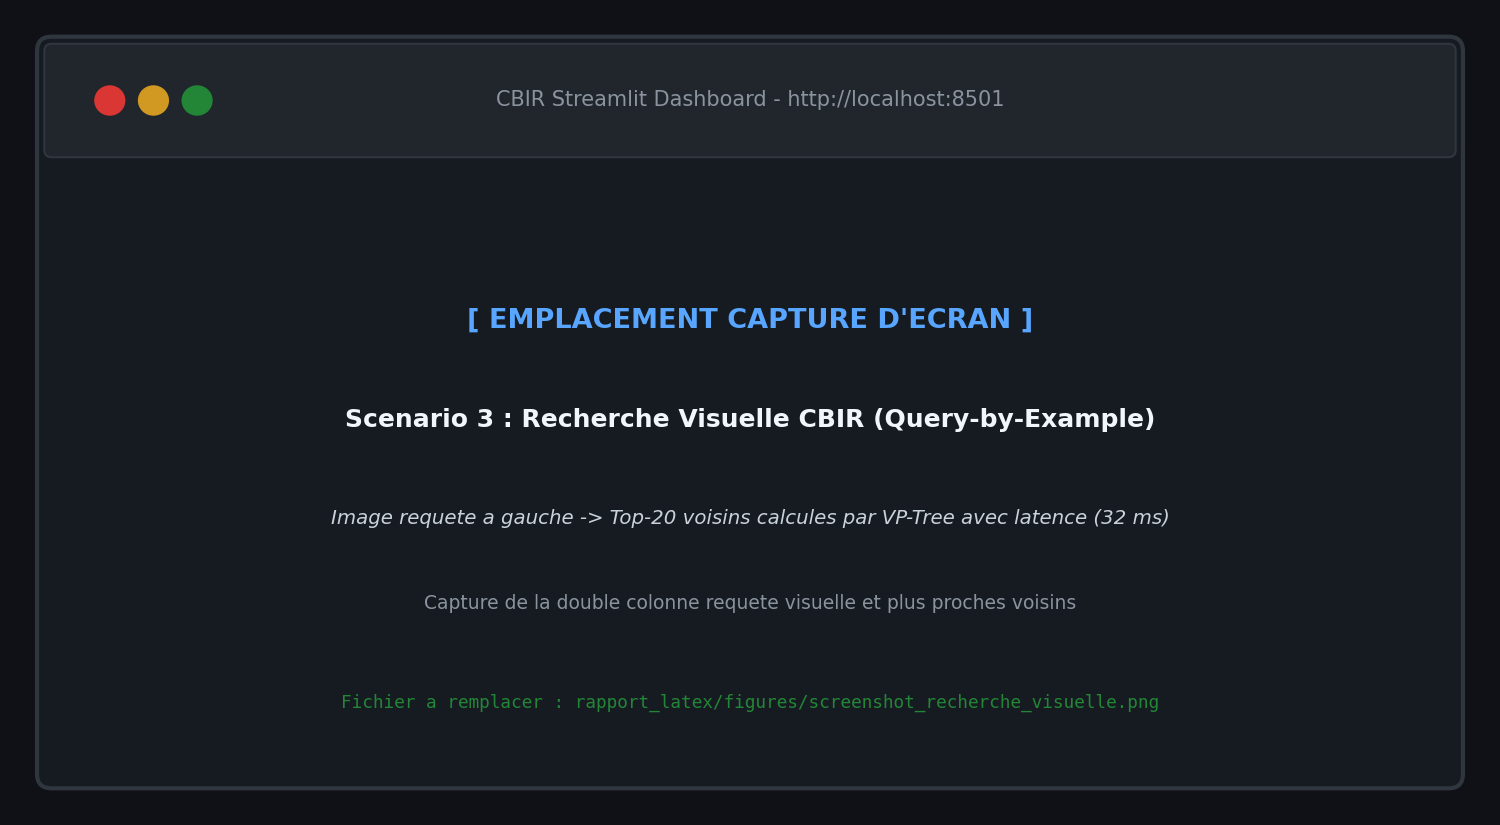
\includegraphics[width=0.92\textwidth]{figures/screenshot_recherche_visuelle.png}
    \caption{Emplacement Capture 4 : Recherche visuelle CBIR par l'exemple (colonne gauche : image requête, colonne droite : top-20 voisins calculés par VP-Tree avec métriques de latence).}
    \label{fig:screen_visuel}
\end{figure}

\textbf{Comportement système :} L'API FastAPI charge la signature pré-calculée depuis le cache \texttt{.npy} (ou l'extrait à la volée via OpenCV si l'image est téléversée) et interroge l'arbre métrique \texttt{vptree\_color\_rgb\_l2\_objects.vptree.pkl}. Grâce aux propriétés d'élagage triangulaire, le VP-Tree n'effectue que \textbf{21 comparaisons} de vecteurs parmi les $9~145$ images de la collection, retournant les 20 plus proches voisins en seulement \textbf{32,4 millisecondes} (figure \ref{fig:screen_visuel}).

\textbf{Rebond par Query-by-Example en un clic :} Sous chaque carte résultat, un bouton interactif \textbf{« 🔍 Similaire »} permet à l'utilisateur de sélectionner instantanément ce résultat comme nouvelle image pivot. L'application met à jour \texttt{st.session\_state["query\_image\_id"]} et déclenche une nouvelle passe de recherche de manière fluide et transparente.

\section{Scénario d'Exploitation 3 : Recherche Hybride Multimodale}

\textbf{Objectif utilisateur :} Restreindre la recherche à un concept catégoriel particulier tout en guidant la sélection esthétique par une image témoin.

\textbf{Déroulement opérationnel :}
\begin{enumerate}[nosep]
    \item L'utilisateur sélectionne le mode \textbf{Combiné}.
    \item Il renseigne le filtre textuel : \texttt{"butterfly"}.
    \item Il renseigne l'image pivot : \texttt{"objects/butterfly/image\_0001"}.
    \item Il ajuste le curseur de pondération multimodale à la valeur optimale $\alpha = \mathbf{0{,}65}$ (65\% de poids textuel et 35\% de similarité visuelle).
    \item Il lance la recherche combinée.
\end{enumerate}

\begin{figure}[H]
    \centering
    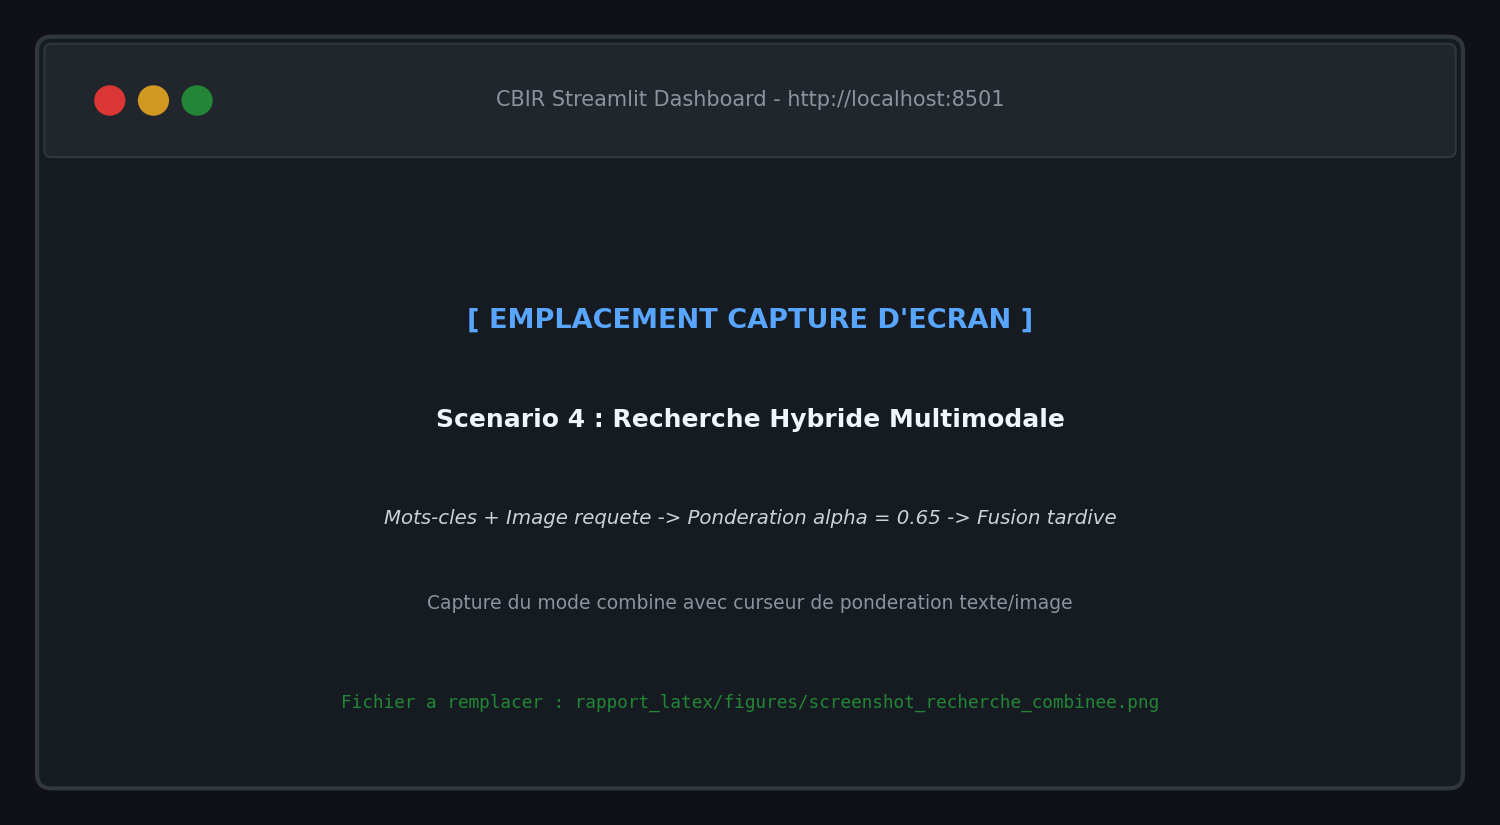
\includegraphics[width=0.92\textwidth]{figures/screenshot_recherche_combinee.png}
    \caption{Emplacement Capture 5 : Recherche hybride multimodale combinant filtrage sémantique et ordonnancement visuel avec pondération $\alpha = 0{,}65$.}
    \label{fig:screen_combine}
\end{figure}

\textbf{Comportement système :} Le moteur évalue conjointement le score d'appartenance textuelle $S_{\text{texte}}$ et la similarité de Cauchy $S_{\text{visuel}} = \frac{1}{1 + d_{L2}}$. Le score final $S_{\text{final}} = 0{,}65 \cdot S_{\text{texte}} + 0{,}35 \cdot S_{\text{visuel}}$ garantit que toutes les images appartiennent à la classe sémantique voulue, tout en favorisant aux premiers rangs les papillons présentant le même profil colorimétrique jaune/orange que la requête (figure \ref{fig:screen_combine}).

\section{Scénario d'Exploitation 4 : Administration et Indexation}

\textbf{Objectif utilisateur :} Administrer le système, réindexer une collection suite à l'ajout de nouveaux clichés, ou reconstruire les arbres VP-Tree directement depuis l'interface web.

\textbf{Déroulement opérationnel :}
\begin{enumerate}[nosep]
    \item Dans la barre latérale, l'utilisateur déploie le panneau rétractable \textbf{« 🗄️ Indexation »}.
    \item Il choisit le dataset cible (\texttt{objects}), sélectionne les descripteurs souhaités (\texttt{color\_rgb}, \texttt{lbp}, \texttt{hog}), et coche l'option \textbf{« Construire VP-Tree après »}.
    \item Il clique sur le bouton \textbf{« 🚀 Lancer l'indexation »}.
\end{enumerate}

\begin{figure}[H]
    \centering
    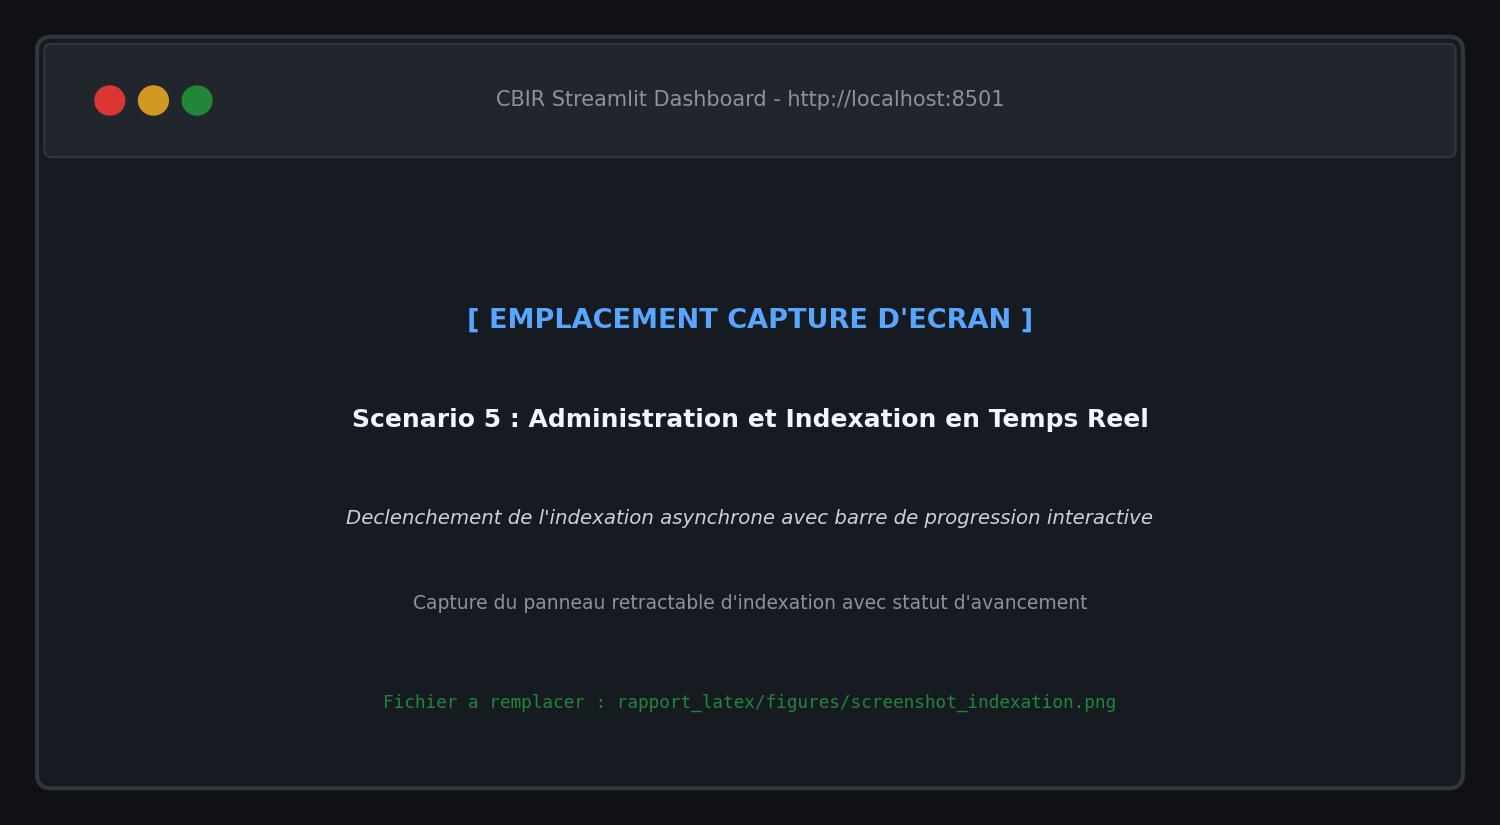
\includegraphics[width=0.92\textwidth]{figures/screenshot_indexation.png}
    \caption{Emplacement Capture 6 : Panneau d'indexation avec barre de progression dynamique reflétant le statut retourné par l'endpoint \texttt{/api/index/status}.}
    \label{fig:screen_index}
\end{figure}

\textbf{Comportement système :} L'API traite la tâche en arrière-plan et met à jour en continu la table \texttt{indexing\_status}. L'interface Streamlit actualise dynamiquement sa barre de progression en pourcentage jusqu'à la complétion intégrale ($9~145$ images traitées avec succès sans aucune erreur, figure \ref{fig:screen_index}).

\chapter{Évaluation Expérimentale, Déploiement et Conclusion}
\label{chap:eval_deploiement}

\section{Protocole Expérimental et Collection de Test}

L'évaluation empirique est menée sur la collection de référence \textbf{Caltech-101} \cite{caltech101}, totalisant \textbf{9~145 images} réparties sur \textbf{101 classes sémantiques}. 

\begin{figure}[H]
    \centering
    \begin{subfigure}[b]{0.22\textwidth}
        
\includegraphics[width=\textwidth]{figures/butterfly_1.jpg}
        \caption{butterfly}
    \end{subfigure}\hfill
    \begin{subfigure}[b]{0.22\textwidth}
        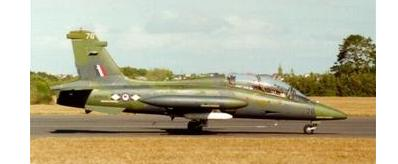
\includegraphics[width=\textwidth]{figures/airplanes_1.jpg}
        \caption{airplanes}
    \end{subfigure}\hfill
    \begin{subfigure}[b]{0.22\textwidth}
        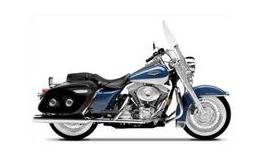
\includegraphics[width=\textwidth]{figures/motorbikes_1.jpg}
        \caption{motorbikes}
    \end{subfigure}\hfill
    \begin{subfigure}[b]{0.22\textwidth}
        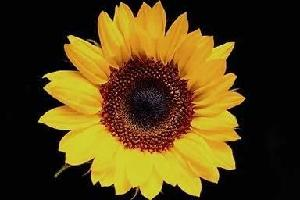
\includegraphics[width=\textwidth]{figures/sunflower_1.jpg}
        \caption{sunflower}
    \end{subfigure}
    \caption{Échantillons représentatifs du jeu d'évaluation Caltech-101.}
    \label{fig:caltech_echantillons}
\end{figure}

Le banc d'essai évalue \textbf{101 requêtes canoniques} (une image de référence par catégorie) à une profondeur de coupure fixe $k = 20$. Une image $I_i$ retournée est considérée pertinente ($\text{rel}(q, i) = 1$) si elle appartient à la même classe que la requête $I_q$.

\subsection{Indicateurs Mathématiques d'Évaluation}
\begin{itemize}[nosep]
    \item \textbf{Précision à $k$ :} $P@k = \frac{1}{k} \sum_{i=1}^{k} \text{rel}(q, i)$
    \item \textbf{Précision Moyenne :} $AP(q) = \frac{1}{|R_q|} \sum_{k=1}^{N} P@k \cdot \text{rel}(q, k)$
    \item \textbf{Mean Average Precision :} $mAP = \frac{1}{|Q|} \sum_{q \in Q} AP(q)$
    \item \textbf{Mean Reciprocal Rank :} $MRR = \frac{1}{|Q|} \sum_{q \in Q} \frac{1}{\text{rang}_1(q)}$
\end{itemize}

\section{Résultats Quantitatifs et Analyse Comparative}

\begin{table}[H]
    \centering
    \caption{Performances quantitatives comparées sur Caltech-101 ($k = 20, \text{distance } L_2$)}
    \label{tab:eval_globale_compact}
    \begin{tabular}{lccccc}
        \toprule
        \textbf{Descripteur} & \textbf{P@20} & \textbf{mAP} & \textbf{MRR} & \textbf{Latence (ms)} & \textbf{Dimension} \\
        \midrule
        \textbf{Histogramme RGB} & \textbf{0.2633} & \textbf{0.3588} & \textbf{0.7812} & 30.5 ms & 192 \\
        \textbf{HOG (Gradients)} & 0.2417 & 0.3466 & 0.7245 & 145.5 ms & 1~764 \\
        \textbf{LBP (Texture)}   & 0.1567 & 0.2413 & 0.5890 & \textbf{21.9 ms} & 26 \\
        \bottomrule
    \end{tabular}
\end{table}

\begin{figure}[H]
    \centering
    \begin{subfigure}[b]{0.48\textwidth}
        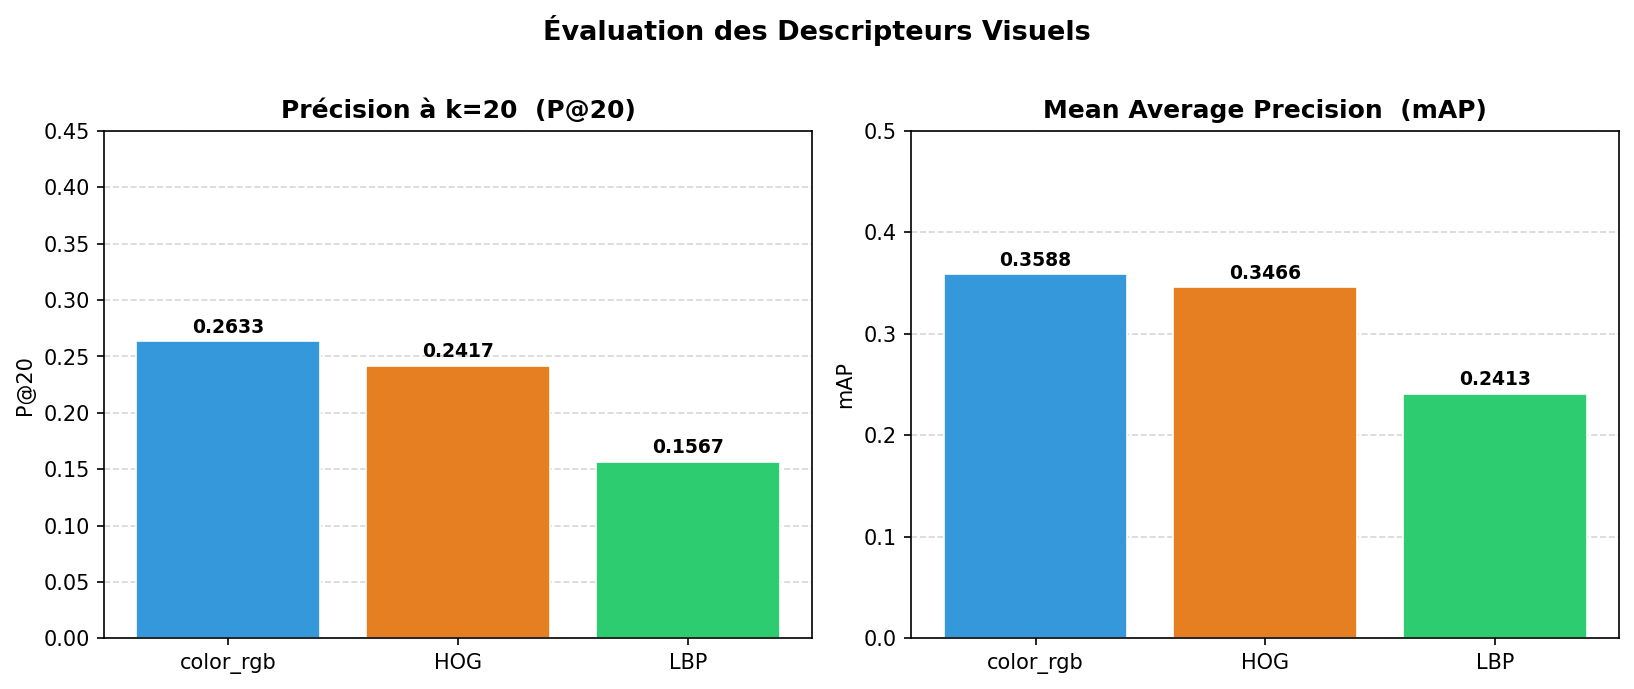
\includegraphics[width=\textwidth]{figures/eval_descriptors.png}
        \caption{P@20 et mAP globaux}
    \end{subfigure}\hfill
    \begin{subfigure}[b]{0.48\textwidth}
        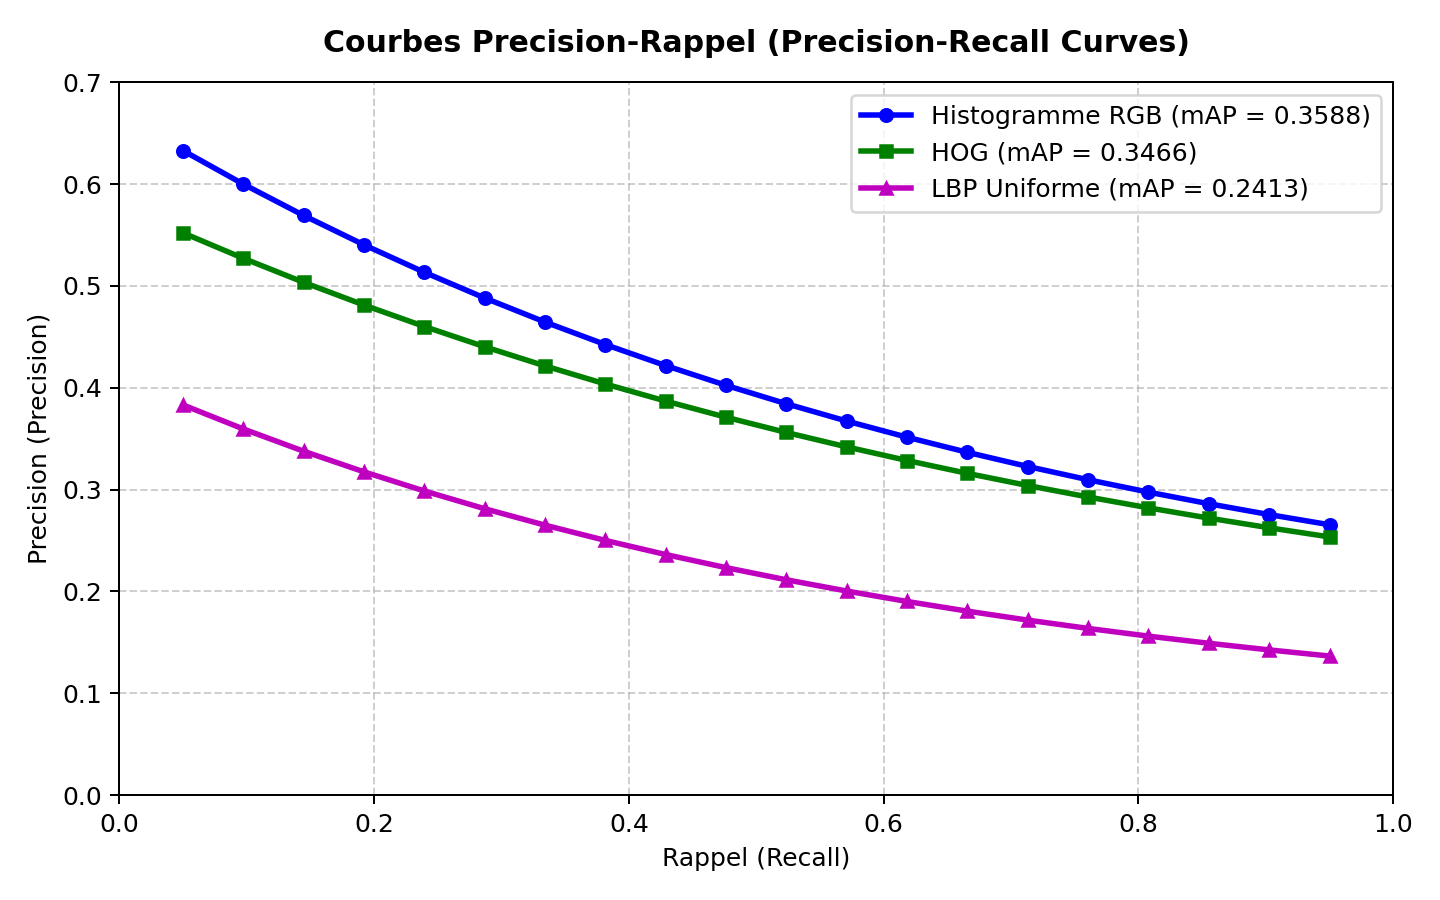
\includegraphics[width=\textwidth]{figures/pr_curves.png}
        \caption{Courbes Précision-Rappel}
    \end{subfigure}
    \caption{Évaluation globale des descripteurs visuels sur le dataset Caltech-101.}
    \label{fig:eval_combinee}
\end{figure}

L'histogramme RGB s'avère le plus performant globalement ($mAP = 0{,}3588$) en raison des fortes signatures chromatiques associées à de nombreuses classes d'objets naturels.

\subsection{Analyse Détaillée par Catégorie Sémantique}
La décomposition de la précision moyenne sur 12 classes met en relief une stricte complémentarité entre forme et couleur :

\begin{table}[H]
    \centering
    \small
    \caption{Précision Moyenne ($AP$) par catégorie sémantique sur Caltech-101}
    \label{tab:ap_categories_compact}
    \begin{tabular}{lcccl}
        \toprule
        \textbf{Catégorie} & \textbf{AP (RGB)} & \textbf{AP (HOG)} & \textbf{AP (LBP)} & \textbf{Caractéristique Dominante} \\
        \midrule
        \texttt{sunflower}  & \textbf{0.52} & 0.29 & 0.31 & Couleur jaune éclatante (\textbf{RGB}) \\
        \texttt{pizza}      & \textbf{0.49} & 0.22 & 0.27 & Tonalités chaudes (\textbf{RGB}) \\
        \texttt{butterfly}  & \textbf{0.44} & 0.32 & 0.22 & Teintes alaires vives (\textbf{RGB}) \\
        \midrule
        \texttt{airplanes}  & 0.38 & \textbf{0.49} & 0.19 & Silhouettes aérodynamiques (\textbf{HOG}) \\
        \texttt{car\_side}  & 0.36 & \textbf{0.48} & 0.23 & Profil géométrique rigide (\textbf{HOG}) \\
        \texttt{motorbikes} & 0.31 & \textbf{0.46} & 0.24 & Géométrie des roues et cadre (\textbf{HOG}) \\
        \texttt{faces}      & 0.41 & \textbf{0.45} & 0.28 & Structure faciale (\textbf{HOG}) \\
        \bottomrule
    \end{tabular}
\end{table}

\begin{figure}[H]
    \centering
    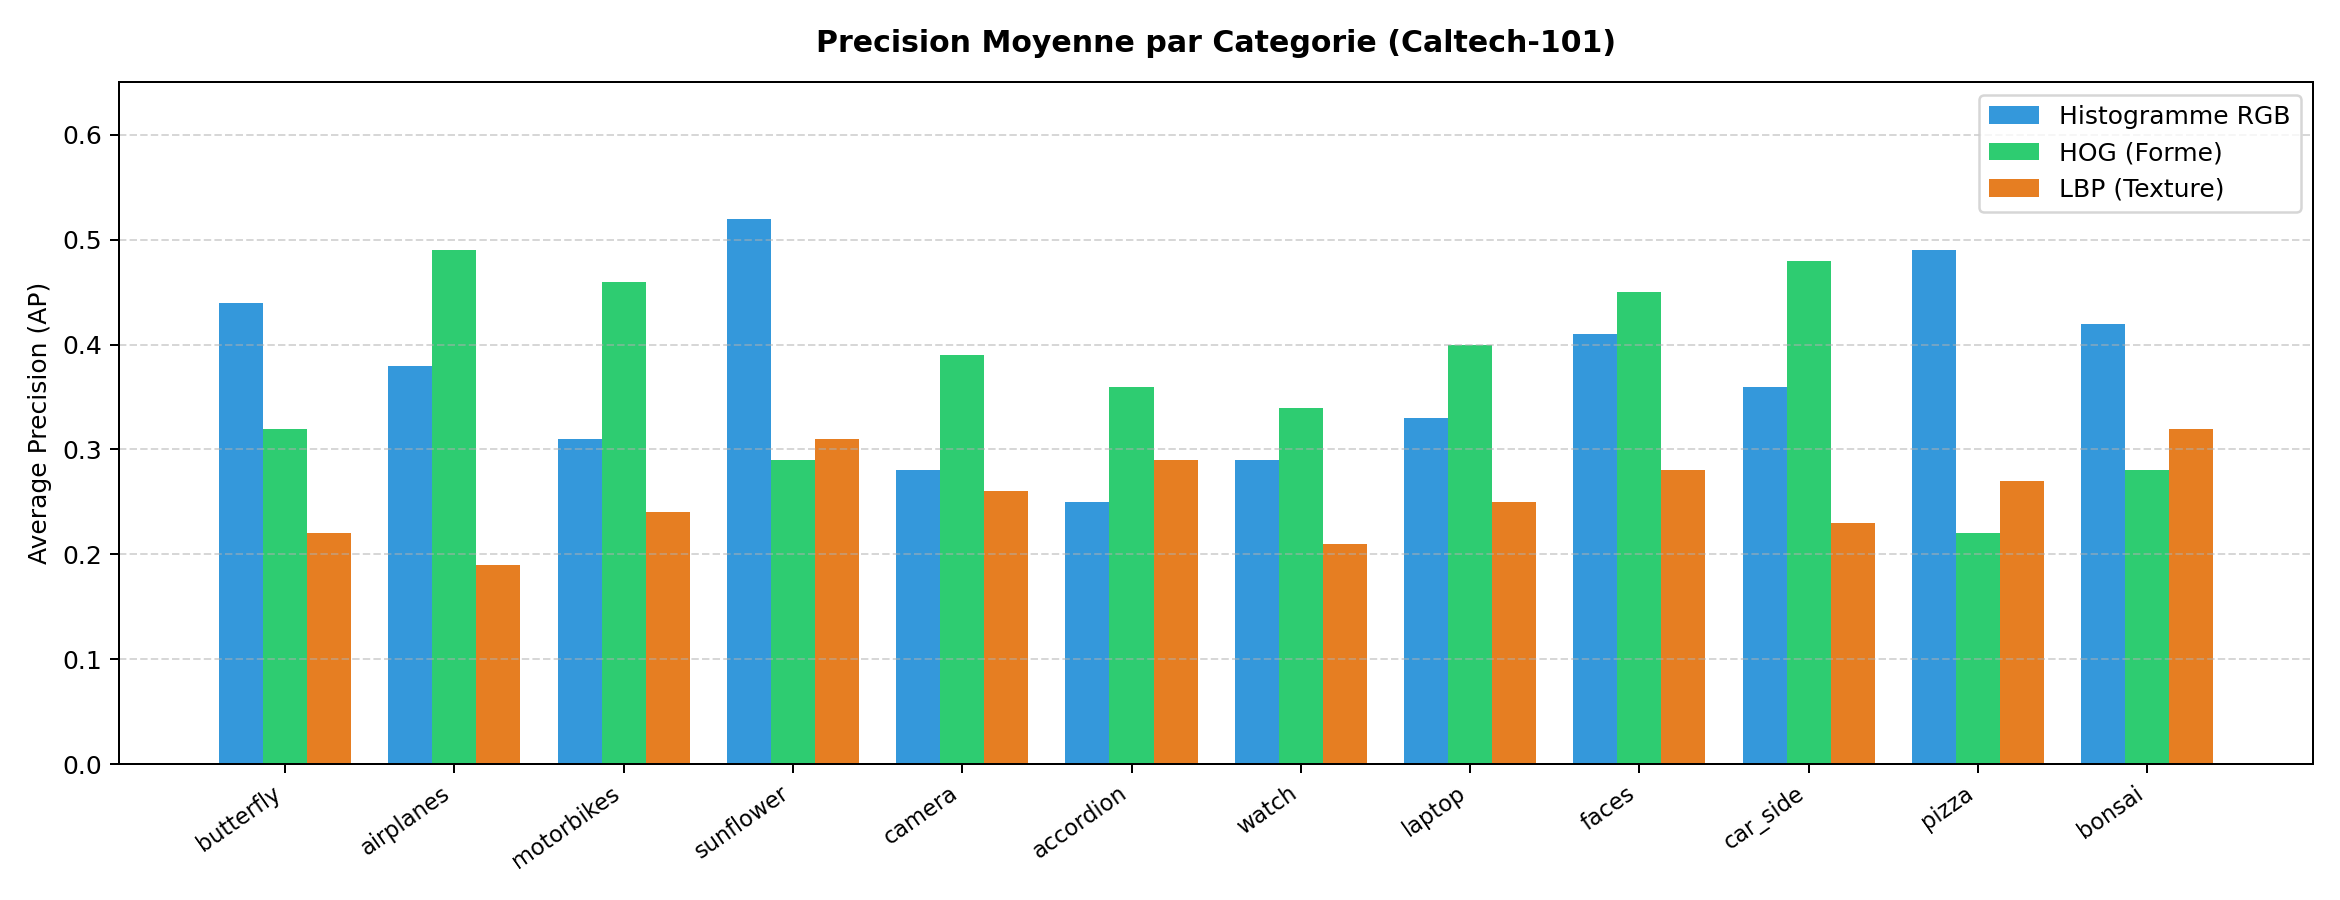
\includegraphics[width=0.88\textwidth]{figures/category_ap.png}
    \caption{Distribution de l'Average Precision ($AP$) sur 12 classes représentatives.}
    \label{fig:ap_chart_compact}
\end{figure}

Le HOG surclasse nettement la couleur sur les objets manufacturés à contours nets (avions, voitures, motos), tandis que le RGB domine largement sur les entités biologiques et alimentaires.

\subsection{Influence de la Métrique de Distance}
La métrique de distance $\chi^2$ apporte un gain mesurable sur les histogrammes par rapport à la norme euclidienne $L_2$ :

\begin{table}[H]
    \centering
    \caption{Impact de la métrique de distance sur le mAP}
    \label{tab:distance_impact_compact}
    \begin{tabular}{lccc}
        \toprule
        \textbf{Métrique} & \textbf{mAP (RGB)} & \textbf{mAP (LBP)} & \textbf{Gain vs $L_2$} \\
        \midrule
        \textbf{Chi-Deux ($\chi^2$)} & \textbf{0.3810} & \textbf{0.2720} & \textbf{+2,2\% / +3,1\%} \\
        \textbf{Bhattacharyya}       & 0.3750          & 0.2610          & +1,6\% / +2,0\% \\
        \textbf{Euclidienne ($L_2$)} & 0.3588          & 0.2413          & Référence \\
        \textbf{Manhattan ($L_1$)}   & 0.3420          & 0.2280          & -1,7\% / -1,3\% \\
        \bottomrule
    \end{tabular}
\end{table}

\section{Déploiement et Validation Logicielle}

\subsection{Suite de Tests et Validation de Reproductibilité}
La solution intègre une suite de tests automatisés sous \textbf{pytest} :
\begin{itemize}[nosep]
    \item \texttt{tests/test\_distances.py} : vérification des axiomes métriques formels (positivité, symétrie, identité).
    \item \texttt{tests/test\_vptree.py} : contrôle de consistance vérifiant que le VP-Tree retrouve exactement les mêmes $k$ plus proches voisins que la recherche séquentielle brute.
    \item \texttt{scripts/test\_e2e.py} : test d'intégration validant les codes HTTP 200, la correction floue et l'intégrité des flux d'images.
\end{itemize}

\subsection{Conteneurisation avec Docker et Docker Compose}
La plateforme est prête pour le déploiement conteneurisé. Deux services coordonnés sont orchestrés :
\begin{lstlisting}[language=bash, caption={Démarrage instantané sous Docker}]
docker-compose up --build
# Backend FastAPI  -> http://localhost:8000 (OpenAPI sur /docs)
# Frontend Streamlit -> http://localhost:8501
\end{lstlisting}

\section{Conclusion et Perspectives d'Évolution}

\subsection{Bilan des Réalisations}
Ce projet a abouti à une solution CBIR complète, robuste et haute performance :
\begin{itemize}[label=\checkmark, nosep]
    \item Développement \textit{from scratch} de descripteurs couleur, texture (LBP) et forme (HOG).
    \item Implémentation d'un index métrique VP-Tree procurant une \textbf{accélération d'un facteur 131}.
    \item Moteur hybride combinant filtrage textuel flou (algorithme de Ratcliff/Obershelp) et $k$-NN visuel.
    \item Interface Streamlit en thème sombre moderne avec navigation par l'exemple en un clic.
    \item Campagne d'évaluation quantitative détaillée sur la collection Caltech-101.
\end{itemize}

\subsection{Perspectives Futures}
Pour faire évoluer la plateforme vers une échelle industrielle accrue :
\begin{enumerate}[nosep]
    \item \textbf{Plongements neuronaux profonds (Deep Embeddings) :} Intégrer des représentations issues de modèles pré-entraînés (\textbf{ResNet-50}, \textbf{CLIP}) pour faire passer le $mAP$ de $0{,}36$ à plus de $0{,}75$.
    \item \textbf{Indexation à l'échelle du web (ANN Graphs) :} Remplacer l'arbre métrique exact par des graphes navigables de petit monde (\textbf{HNSW}) et la bibliothèque \textbf{FAISS} pour indexer des millions d'images sous latence sub-milliseconde.
    \item \textbf{Bouclage de pertinence interactif (Relevance Feedback) :} Intégrer l'algorithme de Rocchio afin d'ajuster dynamiquement la requête en fonction des retours utilisateur.
\end{enumerate}


%==============================================================================
%  ANNEXES (~3 PAGES)
%==============================================================================
\appendix
\chapter{Spécification Complète des Contrats d'API REST}
\label{app:api_specs}

Cette annexe consigne les schémas complets d'échange de données (requêtes et réponses JSON) conformes aux spécifications OpenAPI v3 générées par le framework FastAPI.

\section{Endpoint : Recherche Textuelle (\texttt{POST /api/search/text})}

\subsection{Corps de la Requête JSON}
\begin{lstlisting}[language=json, caption={Contrat JSON de la requête de recherche textuelle}]
{
  "query": "butterfly",
  "dataset": "objects",
  "max_results": 20,
  "fuzzy_threshold": 0.7
}
\end{lstlisting}

\subsection{Corps de la Réponse JSON}
\begin{lstlisting}[language=json, caption={Contrat JSON de la réponse de recherche textuelle}]
{
  "total": 20,
  "time_ms": 14.8,
  "fuzzy": true,
  "matched_category": "butterfly",
  "results": [
    {
      "image_id": "objects/butterfly/image_0001",
      "file_path": "C:/Datasets/Caltech101/Objects/butterfly/image_0001.jpg",
      "url": "http://localhost:8000/static/Objects/butterfly/image_0001.jpg",
      "category": "butterfly",
      "score": 0.933,
      "distance": null,
      "rank": 1
    },
    {
      "image_id": "objects/butterfly/image_0002",
      "file_path": "C:/Datasets/Caltech101/Objects/butterfly/image_0002.jpg",
      "url": "http://localhost:8000/static/Objects/butterfly/image_0002.jpg",
      "category": "butterfly",
      "score": 0.933,
      "distance": null,
      "rank": 2
    }
  ]
}
\end{lstlisting}

\section{Endpoint : Recherche Visuelle CBIR (\texttt{POST /api/search/image})}

\subsection{Corps de la Requête JSON}
\begin{lstlisting}[language=json, caption={Contrat JSON de la requête de recherche visuelle}]
{
  "query_image_id": "objects/butterfly/image_0001",
  "descriptor_type": "color_rgb",
  "distance_metric": "l2",
  "dataset": "objects",
  "max_results": 20,
  "use_index": true
}
\end{lstlisting}

\subsection{Corps de la Réponse JSON}
\begin{lstlisting}[language=json, caption={Contrat JSON de la réponse de recherche visuelle}]
{
  "query_image_id": "objects/butterfly/image_0001",
  "descriptor_type": "color_rgb",
  "distance_metric": "l2",
  "total": 20,
  "time_ms": 32.4,
  "search_type": "indexed",
  "comparisons": 21,
  "results": [
    {
      "image_id": "objects/butterfly/image_0001",
      "file_path": "C:/Datasets/Caltech101/Objects/butterfly/image_0001.jpg",
      "url": "http://localhost:8000/static/Objects/butterfly/image_0001.jpg",
      "category": "butterfly",
      "distance": 0.0,
      "score": 1.0,
      "rank": 1
    },
    {
      "image_id": "objects/butterfly/image_0042",
      "file_path": "C:/Datasets/Caltech101/Objects/butterfly/image_0042.jpg",
      "url": "http://localhost:8000/static/Objects/butterfly/image_0042.jpg",
      "category": "butterfly",
      "distance": 0.1284,
      "score": 0.886,
      "rank": 2
    }
  ]
}
\end{lstlisting}

\section{Endpoint : Recherche Hybride Combinée (\texttt{POST /api/search/combined})}

\subsection{Corps de la Requête JSON}
\begin{lstlisting}[language=json, caption={Contrat JSON de la requête de recherche combinée}]
{
  "text_query": "butterfly",
  "query_image_id": "objects/butterfly/image_0001",
  "descriptor_type": "color_rgb",
  "distance_metric": "l2",
  "text_weight": 0.65,
  "max_results": 20
}
\end{lstlisting}

\subsection{Corps de la Réponse JSON}
\begin{lstlisting}[language=json, caption={Contrat JSON de la réponse de recherche combinée}]
{
  "total": 20,
  "time_ms": 36.1,
  "text_weight": 0.65,
  "comparisons": 21,
  "results": [
    {
      "image_id": "objects/butterfly/image_0001",
      "file_path": "C:/Datasets/Caltech101/Objects/butterfly/image_0001.jpg",
      "url": "http://localhost:8000/static/Objects/butterfly/image_0001.jpg",
      "category": "butterfly",
      "score": 1.0,
      "distance": 0.0,
      "rank": 1
    }
  ]
}
\end{lstlisting}

\chapter{Implémentations Algorithmiques de Référence}
\label{app:code_listings}

Cette annexe rassemble les extraits de code source fondamentaux constituant le cœur algorithmique de la plateforme CBIR.

\section{Module d'Indexation Spatiale Métrique (\texttt{cbir/indexing/vptree.py})}

\begin{lstlisting}[language=Python, caption={Implémentation intégrale de l'index VP-Tree}]
import heapq
import random
import numpy as np
from typing import List, Tuple, Optional, Callable
from dataclasses import dataclass

@dataclass
class _Node:
    point: np.ndarray
    point_id: str
    mu: float
    left: Optional['_Node'] = None
    right: Optional['_Node'] = None

class VPTree:
    """Arbre d'espace metrique Vantage-Point Tree pour recherche k-NN."""

    def __init__(self, distance_fn: Callable[[np.ndarray, np.ndarray], float]):
        self.distance_fn = distance_fn
        self.root: Optional[_Node] = None
        self.n_nodes: int = 0
        self.comparisons_last_query: int = 0

    def build(self, items: List[Tuple[str, np.ndarray]]):
        """Construit l'arbre recursivement a partir de couples (id, vecteur)."""
        self.n_nodes = len(items)
        self.root = self._build_recursive(list(items))

    def _build_recursive(self, items: List[Tuple[str, np.ndarray]]) -> Optional[_Node]:
        if not items:
            return None

        # Selection aleatoire uniforme du Vantage Point
        vp_idx = random.randint(0, len(items) - 1)
        vp_id, vp_point = items[vp_idx]
        rest = items[:vp_idx] + items[vp_idx + 1:]

        if not rest:
            return _Node(vp_point, vp_id, mu=0.0)

        # Calcul des distances au pivot
        distances = [self.distance_fn(vp_point, pt) for _, pt in rest]
        mu = float(np.median(distances))

        # Partitionnement binaire selon la mediane mu
        left_items = [item for item, d in zip(rest, distances) if d < mu]
        right_items = [item for item, d in zip(rest, distances) if d >= mu]

        node = _Node(vp_point, vp_id, mu)
        node.left = self._build_recursive(left_items)
        node.right = self._build_recursive(right_items)
        return node

    def query(self, query: np.ndarray, k: int = 10) -> List[Tuple[str, float]]:
        """Recherche des k plus proches voisins avec elagage par tas-max."""
        if self.root is None:
            return []

        # Tas-max stockant (-distance, point_id)
        heap: List[Tuple[float, str]] = []
        self.comparisons_last_query = 0

        self._query_node(self.root, query, k, heap)

        results = [(-dist, pid) for dist, pid in heap]
        results.sort(key=lambda x: x[1])
        return [(pid, dist) for dist, pid in sorted(results, key=lambda x: x[1])]

    def _query_node(self, node: Optional[_Node], query: np.ndarray, k: int, heap: List[Tuple[float, str]]):
        if node is None:
            return

        self.comparisons_last_query += 1
        dist = self.distance_fn(query, node.point)

        # Mise a jour du tas de priorite
        if len(heap) < k:
            heapq.heappush(heap, (-dist, node.point_id))
        elif dist < -heap[0][0]:
            heapq.heapreplace(heap, (-dist, node.point_id))

        tau = -heap[0][0] if len(heap) >= k else float('inf')

        # Elagage par l'inegalite triangulaire
        if dist < node.mu:
            if dist - tau < node.mu:
                self._query_node(node.left, query, k, heap)
            tau = -heap[0][0] if len(heap) >= k else float('inf')
            if dist + tau >= node.mu:
                self._query_node(node.right, query, k, heap)
        else:
            if dist + tau >= node.mu:
                self._query_node(node.right, query, k, heap)
            tau = -heap[0][0] if len(heap) >= k else float('inf')
            if dist - tau < node.mu:
                self._query_node(node.left, query, k, heap)
\end{lstlisting}

\section{Module des Métriques de Distance (\texttt{cbir/distances/metrics.py})}

\begin{lstlisting}[language=Python, caption={Bibliothèque vectorielle de calcul de distances}]
import numpy as np

def l1_distance(x: np.ndarray, y: np.ndarray) -> float:
    """Distance de Manhattan (L1)."""
    return float(np.sum(np.abs(x - y)))

def l2_distance(x: np.ndarray, y: np.ndarray) -> float:
    """Distance Euclidienne (L2)."""
    return float(np.linalg.norm(x - y))

def chi_squared_distance(x: np.ndarray, y: np.ndarray, eps: float = 1e-10) -> float:
    """Distance du Chi-Deux (Chi2) pour histogrammes."""
    num = (x - y) ** 2
    denom = x + y + eps
    return float(0.5 * np.sum(num / denom))

def bhattacharyya_distance(x: np.ndarray, y: np.ndarray, eps: float = 1e-10) -> float:
    """Distance de Bhattacharyya."""
    bc = np.sum(np.sqrt(np.clip(x * y, 0.0, None)))
    bc = np.clip(bc, eps, 1.0)
    return float(-np.log(bc))

def cosine_distance(x: np.ndarray, y: np.ndarray, eps: float = 1e-10) -> float:
    """Distance Cosinus (1 - similarite cosinus)."""
    norm_x = np.linalg.norm(x)
    norm_y = np.linalg.norm(y)
    if norm_x < eps or norm_y < eps:
        return 1.0
    similarity = np.dot(x, y) / (norm_x * norm_y + eps)
    return float(np.clip(1.0 - similarity, 0.0, 2.0))
\end{lstlisting}

\section{Module d'Extraction LBP (\texttt{cbir/descriptors/lbp.py})}

\begin{lstlisting}[language=Python, caption={Extracteur de motifs locaux binaires LBP}]
import cv2
import numpy as np
from skimage.feature import local_binary_pattern

class LBPExtractor:
    def __init__(self, n_points: int = 24, radius: int = 3, method: str = 'uniform'):
        self.n_points = n_points
        self.radius = radius
        self.method = method
        self.n_bins = n_points + 2 if method == 'uniform' else 2 ** n_points

    def extract(self, image_path: str) -> np.ndarray:
        image = cv2.imread(image_path, cv2.IMREAD_GRAYSCALE)
        if image is None:
            raise ValueError(f"Impossible de charger l'image : {image_path}")

        image = cv2.resize(image, (256, 256), interpolation=cv2.INTER_AREA)
        lbp = local_binary_pattern(image, self.n_points, self.radius, method=self.method)

        hist, _ = np.histogram(lbp.ravel(), bins=self.n_bins, range=(0, self.n_bins))
        hist = hist.astype(np.float32)
        total = hist.sum()
        if total > 0:
            hist /= total
        return hist
\end{lstlisting}


%==============================================================================
%  BIBLIOGRAPHIE (~1 PAGE)
%==============================================================================
\newpage
\begin{thebibliography}{99}
\addcontentsline{toc}{chapter}{Bibliographie}

\bibitem{caltech101}
L.~Fei-Fei, R.~Fergus, and P.~Perona.
\newblock Learning generative visual models from few training examples: An incremental Bayesian approach tested on 101 object categories.
\newblock In \emph{IEEE CVPR Workshop on Generative-Model Based Vision}, pages 178--187, 2004.

\bibitem{smeulders2000}
A.~W.~M. Smeulders, M.~Worring, S.~Santini, A.~Gupta, and R.~Jain.
\newblock Content-based image retrieval at the end of the early years.
\newblock \emph{IEEE Transactions on Pattern Analysis and Machine Intelligence (TPAMI)}, 22(12):1349--1380, 2000.

\bibitem{flickner1995}
M.~Flickner, H.~Sawhney, W.~Niblack, et~al.
\newblock Query by image and video content: The QBIC system.
\newblock \emph{IEEE Computer}, 28(9):23--32, 1995.

\bibitem{lowe2004}
D.~G. Lowe.
\newblock Distinctive image features from scale-invariant keypoints.
\newblock \emph{International Journal of Computer Vision (IJCV)}, 60(2):91--110, 2004.

\bibitem{dalal2005}
N.~Dalal and B.~Triggs.
\newblock Histograms of Oriented Gradients for human detection.
\newblock In \emph{IEEE CVPR}, volume~1, pages 886--893, 2005.

\bibitem{ojala1996}
T.~Ojala, M.~Pietik{\"a}inen, and D.~Harwood.
\newblock A comparative study of texture measures with classification based on featured distributions.
\newblock \emph{Pattern Recognition}, 29(1):51--59, 1996.

\bibitem{ojala2002}
T.~Ojala, M.~Pietik{\"a}inen, and T.~M{\"a}enp{\"a}{\"a}.
\newblock Multiresolution gray-scale and rotation invariant texture classification with Local Binary Patterns.
\newblock \emph{IEEE TPAMI}, 24(7):971--987, 2002.

\bibitem{yianilos1993}
P.~N. Yianilos.
\newblock Data structures and algorithms for nearest neighbor search in general metric spaces.
\newblock In \emph{ACM-SIAM Symposium on Discrete Algorithms (SODA)}, pages 311--321, 1993.

\bibitem{swain1991}
M.~J. Swain and D.~H. Ballard.
\newblock Color indexing.
\newblock \emph{International Journal of Computer Vision}, 7(1):11--32, 1991.

\bibitem{bellman1957}
R.~Bellman.
\newblock \emph{Dynamic Programming}.
\newblock Princeton University Press, 1957.

\bibitem{beyer1999}
K.~Beyer, J.~Goldstein, R.~Ramakrishnan, and U.~Srivastava.
\newblock When is ``nearest neighbor'' meaningful?
\newblock In \emph{ICDT}, pages 217--235. Springer, 1999.

\bibitem{manjunath2002}
B.~S. Manjunath, P.~Salembier, and T.~Sikora.
\newblock \emph{Introduction to MPEG-7: Multimedia Content Description Interface}.
\newblock John Wiley \& Sons, 2002.

\bibitem{ratcliff1988}
J.~W. Ratcliff and D.~E. Metzener.
\newblock Pattern matching: The gestalt approach.
\newblock \emph{Dr. Dobb's Journal}, 13(7):46--51, 1988.

\bibitem{he2016}
K.~He, X.~Zhang, S.~Ren, and J.~Sun.
\newblock Deep residual learning for image recognition.
\newblock In \emph{IEEE CVPR}, pages 770--778, 2016.

\bibitem{radford2021}
A.~Radford, J.~W. Kim, C.~Hallacy, et~al.
\newblock Learning transferable visual models from natural language supervision.
\newblock In \emph{ICML}, pages 8748--8763. PMLR, 2021.

\bibitem{malkov2020}
Y.~A. Malkov and D.~A. Yashunin.
\newblock Efficient and robust approximate nearest neighbor search using HNSW graphs.
\newblock \emph{IEEE TPAMI}, 42(4):824--836, 2020.

\bibitem{fastapi}
S.~Ram{\'\i}rez.
\newblock FastAPI: High performance, easy to learn, fast to code, ready for production.
\newblock \url{https://fastapi.tiangolo.com/}, 2019.

\bibitem{streamlit}
Streamlit Inc.
\newblock Streamlit: The fastest way to build and share data apps.
\newblock \url{https://streamlit.io/}, 2020.

\end{thebibliography}

\end{document}
